\chapter{Double zero MVDR ABF}% for notch broadening}
\label{ch:dzmvdr}
ABFs encounter interferer direction mismatch because of interferer
motion or limited sample support available to compute the SCM
\cite{vtree2002oap}. This mismatch results in a loss of interferer
suppression and degraded output performance. Notch broadening is a
robust beamforming technique to address interferer mismatch by
creating wider beampattern notch in the interferer direction. This
chapter presents a new ABF approach for notch broadening. The double
zero MVDR (DZ MVDR) ABF exploits the properties of the array
polynomial zeros to create broad notch in the interferer
direction. The DZ MVDR ABF assumes using a ULA similarly to the UC
MVDR ABF, but does not necessarily assume that the observed snapshots are
plane waves. The first two sections of this chapter introduces the
interferer mismatch problem and the notch broadening technique for
robust beamforming. \sect{}~\ref{sec:second-order-zeros} discusses the
behavior of ABF beampattern in the vicinity of a null.
\sect{}\ref{sec:double-zero-mvdr} describes the DZ MVDR
algorithm. \sect{}\ref{sec:results} presents results of experiments
evaluating the DZ MVDR ABF in both stationary and moving interferer
scenarios. 

\section{Interferer mismatch}
\label{sec:interferer-mismatch}
ABFs place sharp and deep notches in the expected interferer direction
to suppress interferer power at the output. However in applications
involving interferer motion or limited snapshot support, the ABFs
suffer from interferer mismatch, i.e., the expected interferer
direction is different from the true interferer direction
\cite{vtree2002oap, riba1997comm, baggeroer1999passive}. Due to this
mismatch in interferer direction, the ABFs place a deep notch in a
direction different from the true interferer direction. As a result,
the ABF produces a shallower notch in the true interferer direction
which does not sufficiently attenuate the interferer. Hence,
interferer direction mismatch results in degraded notch depth (ND) in
the interferer direction and subsequent loss of suppression.

In a dynamic environment, moving interferers may traverse several
resolution widths during the snapshot averaging interval
\cite{baggeroer1999passive}. The motion spreads the interferer power
into multiple eigenvalues of the SCM. The number of dominant
eigenvalues is approximately equal to the number of resolution width
($\resW$) traversed by the interferer
\cite{cox2000mrabf}. Effectively, a single source appears to split
into multiple spatially separate sources. This source splitting due to
interferer motion results in interferer direction mismatch when
implementing the SCM based ABFs. In a snapshot limited scenario
($L \approx N$), random matrix theory based analysis show that the
dominant eigenvectors of the SCM are biased estimates of the dominant
eigenvectors of the ECM \cite{paul2007asymptotics,
  benaych2011eigen}. When the observed snapshots consist of planewave
interferers in white background noise, the dominant eigenvectors
represent the interferers that need to be suppressed
\cite{vtree2002oap}. However, due to the biased estimate of the
dominant eigenvectors, an ABF implemented using the SCM suffers from
the interferer direction mismatch. As discussed above, the interferer
mismatch leads to degraded notch depth in the interferer direction and
subsequent loss of interferer power suppression using ABFs.

\section{Notch broadening}
\label{sec:notch-broadening}
Beampattern notch broadening is a robust beamforming technique that
addresses the interferer mismatch problem arising from interferer
motion and the limited snapshot condition \cite{vtree2002oap}. A broad
notch in the interferer direction can continue to suppress the
interferer even in the case of a mismatch. One approach to notch
broadening is covariance augmentation method which modifies the SCM
such that the resulting ABF creates broad interferer notches
\cite[Sec.~6.7.6]{vtree2002oap}. Riba et al. proposed a notch
broadening technique by modifying the SCM using a 'spreading matrix'
\cite{riba1997comm}. The beamformer was designed for mobile
communication environment with fast moving interferers. Zatman and
Mailloux independently proposed separate but related methods to
produce broad notches in the MVDR beampattern \cite{zatman1995null,
  mailloux1995null}. Both methods modify the SCM to introduce a
cluster of incoherent fictitious sources around each of the original
interferer direction. The fictitious sources are introduced by
modifying the SCM prior to computing the MVDR weights. The resulting
MVDR weights places a null in the vicinity of each fictitious source,
producing a wide notch region around the interferer direction. Later,
Guerci combined the two methods under the theory of covariance matrix
tapering (CMT) for notch broadening \cite{guerci1999cmt}. The CMT
approach uses a spatially tapered SCM to compute the MVDR ABF weights
which produces broad notches in the interferer direction. The CMT
approach for notch broadening is discussed in the next section.

Another approach is to impose constraints on the derivatives of the
beampattern in the interferer direction
\cite[Sec.~6.7.1.4]{vtree2002oap}. This approach computes the MVDR ABF
weights with the constraint of the derivative of the beampattern
function $\beampatu$ with respect to directional cosine $u$ set to a
specified value at the interferer direction $\uinter$. The derivative
constraint forces the beampattern at the interferer directions, i.e.,
the notches to be flatter and broader. Gershman used the
derivative constraint approach to produce notch broadening in the MVDR ABF
beampattern. Gershman's method sets the beampattern derivatives at all
the interferer directions to zero \cite{gershman1991synthesis}. The
method does not require \emph{a priori} knowledge of interferer
direction, however the method assumes either a high power interferer
or a large number of snapshots available to estimate the SCM
accurately. Such assumption of large snapshot support is suitable only
in electromagnetic waves based applications but is unrealistic in most
passive sonar applications \cite{baggeroer1999passive}.

\subsection{Covariance matrix tapering}
\label{sec:cmt}
Guerci proposed the CMT approach for notch broadening in ABF
beampatterns \cite{guerci1999cmt}. The CMT technique augments the SCM
using a taper matrix $\taperMat$ to generate the tapered SCM
$\sampCov_{\rm T} = \sampCov\circ\taperMat$, where $[\circ]$ denotes
the Hadamard matrix product. The taper matrix $\taperMat$ is a
positive semi-definite (p.s.d) matrix with all the main diagonal
entries equal to unity. The p.s.d taper matrix ensures that the
tapered SCM is also p.s.d and the unity diagonal entries ensures that
$\tr{\sampCov_{\rm T}} = \tr{\sampCov}$, i.e., the tapering conserves
the total input power in the SCM. The CMT MVDR ABF weight vector is
computed by replacing the ECM with the tapered SCM $\sampCov_{\rm T}$
in \eqref{eq:mvdr-wt}. The ABF weight vector computed using the
tapered SCM produces broad notches in the interferer direction
compared to the SMI MVDR ABF. The choice of the taper matrix
$\taperMat$ determines the shape and width of the broadened notch. The
simplest choice for the taper matrix $\taperMat$ has the entries,
\begin{equation}
  \label{eq:taper-mat}
[\taperMat]_{mn} = {\rm sinc}((m - n)\cmtW/2)  
\end{equation}
where the parameter $\cmtW$ defines the desired notch width in terms
of directional cosine. Using the taper matrix in \eqref{eq:taper-mat}
creates a uniform notch of width $\cmtW$ centered at the interferer
direction. Unlike the Zatman and Mailloux approach, the CMT approach
does not require prior knowledge of the interferer direction, but it
requires choosing the notch width parameter $\cmtW$ before
implementation. The choice of the width parameter depends on the
application environment which is usually unknown a priori. In a
passive sonar application scenario, Song suggests that an appropriate
choice for the notch width is equal to the resolution width for the
given array aperture, i.e., $\cmtW = 2/(N-1)$ \cite{song2003null}.

\begin{figure}[!ht]
  \centering
\subfloat[]{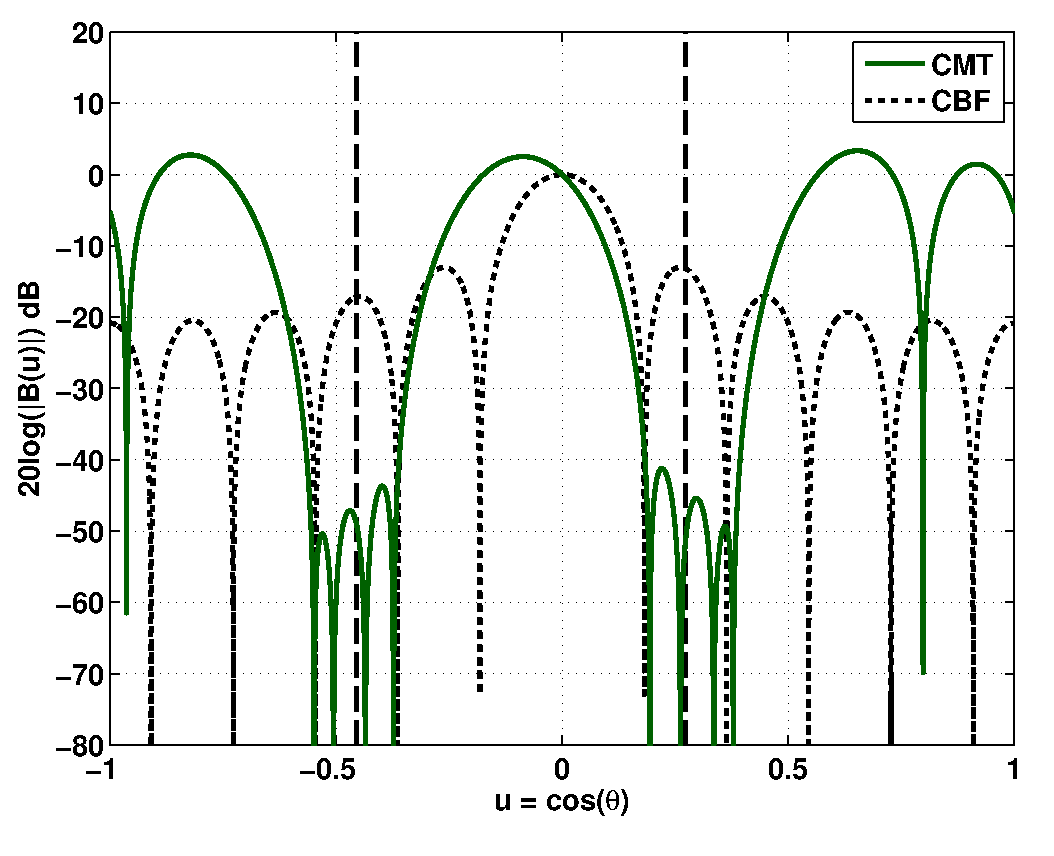
\includegraphics[width=0.6\textwidth]{cmt_bp.pdf}\label{fig:cmt-bp}}

\subfloat[]{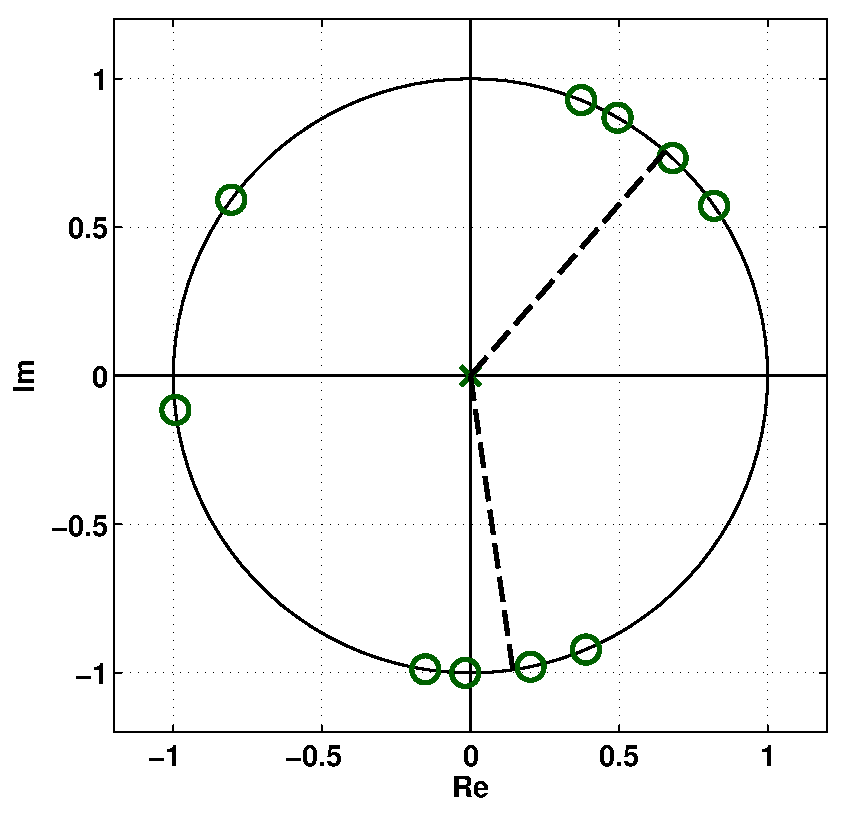
\includegraphics[width=0.6\textwidth]{cmt_pz.pdf}\label{fig:cmt-pz}}

\caption[(a) Log-magnitude beampattern and (b) zeros of CMT MVDR ABF
  using $N = 11$ sensor ULA and steered towards $\ulook = 0$.]{(a) Log-magnitude beampattern and (b) zeros of CMT MVDR ABF
  using $N = 11$ sensor ULA and steered towards $\ulook = 0$. The CMT
  notch width $\cmtW = 2/(N-1$). Two interferers are present at
  directions $\uinter = 3/N$ and $-5/N$ denoted by dashed vertical
  lines in (a) and dashed radial lines in (b). The CMT MVDR uses four
  zeros per interferer to create broad notch at the cost of high
  sidelobes and wider mainlobe.}
\label{fig:cmt-bp-pz}
\end{figure}

\figurename{}~\ref{fig:cmt-bp-pz} shows the log-magnitude beampattern
(top panel) and the polynomial zeros (bottom panel) of a CMT MVDR ABF
(solid green) implemented using $N = 11$ sensor ULA assuming the ECM
is known. A CBF beampattern (dotted black) is also shown for
reference. Two independent interferers are present at $\uinter = 3/N$
and $-5/N$ respectively as denoted by the vertical dashed lines in
beampattern and radial dashed lines in zeros plot. The CMT notch width
is set to $\cmtW = 2/(N-1)$. Examining the beampattern, the CMT MVDR
ABF produces broad notch at each interferer direction. The notch
broadening is achieved by clustering multiple beampattern nulls in the
vicinity of the interferer direction. Equivalently, the associated CMT
MVDR polynomial zeros cluster in the vicinity of a interferer
direction, as seen in the zeros plot. For a given interferer strength,
the number of zeros used to produce the notch broadening depends on
the notch width parameter $\cmtW$. The wider the notch width required,
more zeros per interferer are used to produce notch broadening. In the
\figurename{}~\ref{fig:cmt-pz}, the CMT MVDR ABF is using four zeros
per interferer to produce broad notches. However, as seen in the
beampattern the CMT MVDR ABF produces broad notches at the cost of
high sidelobes and wider mainlobe which reduces the WNG
[\sect{}\ref{sec:white-noise-gain}].

\subsubsection{CMT as spatial modulation}
\label{sec:cmt-as-spatial}
CMT approach using taper matrix $\taperMat$ in \eqref{eq:taper-mat}
generates fictitious sources around the interferer direction as
discussed below. The eigendecomposition of the taper matrix is
$\taperMat = \sum_{n=1}^{N}\eval_n\taperevec_n\taperevec_n\herm$ where
$\taperevec_n$ is the $n\nth$ eigenvector and $\eval_n$ is the
associated eigenvalue such that
$\eval_1 \geq \eval_2 \geq \ldots \eval_N$. The number of significant
eigenvalues of the taper matrix in \eqref{eq:taper-mat} is
$\cmtW(N-1)/2 + 1$ \cite{song2003null}. Hence, for a notch width of
$W = 2/(N-1)$, the taper matrix $\taperMat$ has only two significant
eigenvalues. Using the eigendecomposition of $\taperMat$, the tapered
SCM is
\begin{align*}
  \sampCov_{T} &= \left( \frac{1}{L}\sum\limits_{\ell = 1}^{L}\datavec_{\ell}\datavec_{\ell}\herm \right) \circ \left( \sum\limits_{n=1}^{N}\eval_n\taperevec_n\taperevec_n\herm \right)\\
 \
 &= \frac{1}{L}\sum\limits_{n=1}^{N}\eval_n\sum\limits_{\ell = 1}^{L}(\datavec_{\ell}\circ\taperevec_n)(\datavec_{\ell}\circ\taperevec_n)\herm\\
               &=
               \sum\limits_{n=1}^{N}\eval_n\left(\frac{1}{L}\sum\limits_{\ell
                 = 1}^{L}\modvec_{n\ell}\modvec_{n\ell}\herm \right ), \\
\intertext{considering only the two significant eigenvalues,}
\sampCov_{T}  &= \sum\limits_{n=1}^{2}\eval_n\sampCov_n,
\end{align*}
where $\modvec_{n\ell} = (\datavec_{\ell}\circ\taperevec_n)$ is the
$\ell\nth$ snapshot $\datavec_{\ell}$ element-wise multiplied by the
eigenvector $\taperevec_n$ and $\sampCov_n$ is the SCM obtained by
averaging $\modvec_{n\ell}$ for $n = 1, 2$. Multiplying a snapshot
$\datavec_{\ell}$ by an eigenvector corresponds to the convolution in
spatial frequency domain between the spatial spectrum of the snapshot
and the eigenbeam, i.e., the spatial spectrum of the eigenvector. A
snapshot $\datavec_{\ell}$ containing stationary planewave interferers
has impulses in the spatial spectrum at interferer directions. Hence,
convolution with interferer spatial spectrum shifts the eigenbeams to
the interferer direction. This is analogous to the classic time domain
amplitude modulation where a sinusoidal carrier is multiplied with the
message signal. The sinusoidal carrier has two impulses in the
frequency domain and convolution with this spectrum makes frequency
shifted copies of the message signal spectrum.

\figurename{}~\ref{fig:cmt-eigenbeam} shows the magnitude of the
eigenbeams of the first two principal eigenvectors $\taperevec_1$
(blue) and $\taperevec_2$ (green). Firstly, the eigenbeam for
$\taperevec_1$ has a single mainlobe in the broadside direction,
identical to the spatial spectrum of a single planewave signal
observed using a ULA. Convolving the snapshot spatial spectrum with
the eigenbeam of $\taperevec_1$ shifts the blue eigenbeam to the
interferer direction. The single mainlobe of the shifted eigenbeam
indicates the interferer signal in the snapshot. Secondly, the
eigenbeam for $\taperevec_2$ has two distinct peaks on either side of
the broadside direction. Convolving the snapshot spatial spectrum with
the eigenbeam of $\taperevec_2$ shifts the the green eigenbeam to
interferer direction. The two peaks of the shifted eigenbeam indicates
a pair of planewave signals on either side of the interferer
direction. In effect, CMT operation performs spatial modulation of the
snapshots $\datavec_{\ell}$ to add a pair of fictitious sources around
the interferer direction resulting in three virtual interferers for
MVDR to suppress for each physical interferer. Hence, an MVDR ABF
implemented using the tapered SCM $\sampCov_{T}$ places notch on
either side of the interferer direction, effectively producing a
broader notch as seen in \figurename{}~\ref{fig:cmt-bp}. Consequently,
the CMT MVDR ABF using notch width $\cmtW = 2/(N-1)$ uses three degree
of freedom (DoF) per interferer to produce notch broadening.

\begin{figure}[!htb]
  \centering
  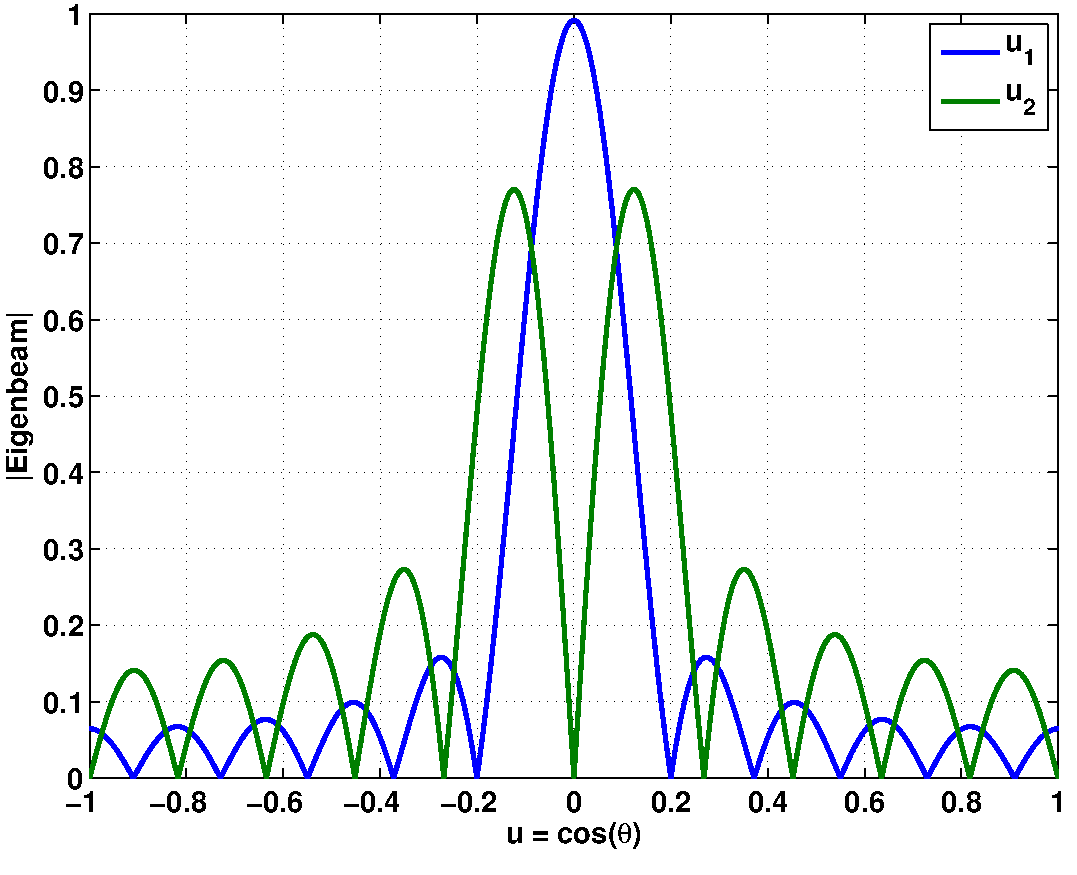
\includegraphics[width=0.8\textwidth]{cmt_eigval_beam.pdf}
  \caption[Magnitude of eigenbeam for first two principal eigenvectors
  of the sinc taper matrix in \eqn{}\eqref{eq:taper-mat}.]{Magnitude
    of eigenbeam for first two principal eigenvectors of the sinc
    taper matrix in \eqn{}\eqref{eq:taper-mat}. The eigenvectors
    spatially modulate the snapshots to create replica of planewave
    signal in the snapshot on either side of the signal direction.}
  \label{fig:cmt-eigenbeam}
\end{figure}

\section{Properties of the beampattern near a zero}
\label{sec:second-order-zeros}
Evaluating the array polynomial \eqref{eq:beampat-poly} on the unit
circle $z = e^{j\pi u}$ yields the beampattern in
\eqref{eq:beampatu}. The array polynomial $\beampolyz{}$ has $N - 1$
zeros in the complex plane and the zeros that fall on the unit circle
produce nulls in the beampattern. A first-order zero on the unit
circle produces a `sharp' null in the beampattern. The beampattern in
the neighborhood of a first-order null is linear in the directional
cosine $u$ \cite[Sec.~3.2.3]{vtree2002oap}\cite{Steinberg1976}. In contrast, the
second-order zeros (SOZ) produce flatter nulls in the beampattern. The
beampattern in the neighborhood of a second-order null is quadratic in
directional cosine $u$. \figurename{}~\ref{fig:mvdr-null-zero}
compares the MVDR beampattern magnitude in the neighborhood of a first-order
null (blue solid) and a second-order null (red dashed). The SOZ effectively
imposes a first derivative constraint on the beampattern which forces
the second-order null to be flatter compared to the sharp first-order
null.

As previously discussed, the ensemble MVDR beamformer places a
beampattern null in the neighborhood of the true interferer direction
to attenuate the interferer. The vertical dashed line in
\figurename{}~\ref{fig:mvdr-null-zero} denotes the interferer
direction $\uinter$. The interferer falls on the 'shoulder' of the
null where the first-order null creates a sharp notch whereas the
second-order null creates a deeper and broader notch. Any mismatch in
the interferer direction changes the ND at the interferer direction
$\uinter$. In case of a mismatch, the ND produced by the first-order
null exhibits greater variation compared to the second-order null due
to the linear and quadratic nature of their respective
beampatterns. As a result, the ND produced by the first-order null is
more sensitive to interferer direction mismatch compared to the ND
produced by the second-order null. The DZ MVDR ABF presented in the
next section exploits this property of a second-order null to produce
broader notches in the MVDR beampattern.

\begin{figure}[!hp]
  \centering
  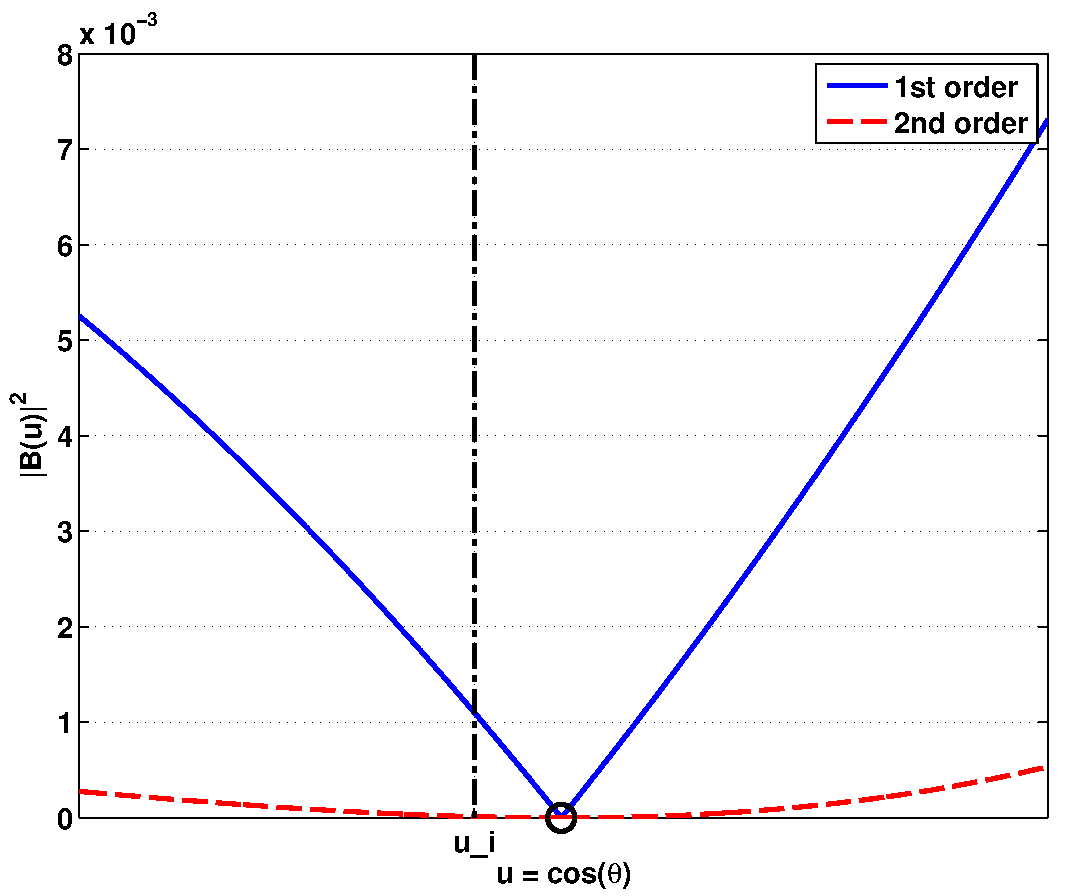
\includegraphics[width=0.8\textwidth]{interf_single_dbl_zero_beampattern.pdf}
  \caption[MVDR beampattern magnitude zoomed into the neighborhood of
    a null.]{MVDR beampattern magnitude zoomed into the neighborhood of
    a null. The null location in directional cosine $u$ axis is
    denoted by the circle marker.  The vertical dashed line indicates
    the interferer direction. The blue solid curve denotes the first
    order null produced by the MVDR beamformer. The red dashed curve
    denotes a second order null in the same location.}
  \label{fig:mvdr-null-zero}
\end{figure}

% ==========================================
% Include files 

\section{Double Zero MVDR ABF}
\label{sec:double-zero-mvdr}
The double zero MVDR (DZ MVDR) ABF is designed to produce broad
beampattern notch in the interferer direction. The DZ MVDR algorithm
exploits the property of the SOZs of array polynomial to produce broad beampattern notches. The flow
diagram \figurename{}~\ref{fig:flow} provides an overview of the DZ
MVDR algorithm. The following section describes the DZ MVDR ABF
algorithm assuming the number of sensors $N$ is odd. The algorithm
extends naturally when $N$ is even by including an additional zero at
$u = 1$ as constrained by even symmetry even length array weights.

\subsection{Algorithm}
\label{sec:algorithm}
The DZ MVDR ABF begins with $L$ data snapshots from an $N$ element
ULA, represented as a data matrix $\dataMat{}$ of dimension
$N \times L$.  The data matrix $\dataMat{}$ is partitioned to create
two submatrices $\dataSubMat{{\rm a}} = \dataMat{(1:K, 1:L)}$ and
$\dataSubMat{\rm b} = \dataMat{(K:N, 1:L)}$ where $K = (N + 1)/2$. The
indices in the subscript of $\dataMat{}$ indicate the range of rows
and columns of $\dataMat{}$ assigned to each submatrix. This
partitioning of the data matrix is equivalent to partitioning the $N$
element full ULA into two $K$ element
subarrays shown in \figurename{}~\ref{fig:subarray}. The $(K-1)\nth$ sensor denoted by white circle is used in both subarrays. The submatrices $\dataSubMat{{\rm a}}$ and
$\dataSubMat{{\rm b}}$ are combined to create an augmented data matrix
$\dataMatK = [\dataSubMat{{\rm a}} | \dataSubMat{{\rm b}}]$ of
dimension $K \times 2L$. The data matrix $\dataMatK$ can be
interpreted as the collection of $2L$ snapshot observed by $K$ element
ULA.

The augmented data matrix is used to compute the subarray SCM
$\sampCov_{\rm K} = (\dataMatK\dataMatK\herm)/(2L)$ and subsequently
the ABF weight vector for a $K$ element subarray
\begin{equation}
  \label{eq:subarray-wt}
  \wtK = \frac{\sampCov_{K}\inv\rep_{K}}{(\rep_{K}\herm \sampCov_{K}\inv\rep_{K})}
\end{equation}
where $\rep_{K}$ is an array manifold vector in the look direction for
the $K$ element subarray. The beamformer in \eqref{eq:subarray-wt} can
be implemented as a SMI MVDR ABF on a $K$ element ULA. The DZ MVDR ABF
weight vector for the full ULA is obtained by convolving the weight vector
$\wtK$ with itself
\begin{equation}
  \label{eq:wt-convo}
  \wtdz = \wtK*\wtK
\end{equation}
where [*] denotes discrete convolution operation considering the weight vector
$\wtK$ as a discrete sequence of length $K$. The resulting DZ MVDR ABF
weight vector $\wtdz$ is of length $2K - 1 = N$.

 The z-transform of \eqref{eq:subarray-wt} yields the array polynomial of
 the subarray SMI MVDR ABF weight vector,
\begin{equation}
  \label{eq:subarray-poly}
  \beampolyz{{\rm K}} = \ztrans{(\wtK)} = G_K\prod_{i=1}^{K - 1}( 1 -
  \sampz_{Ki} z\inv).
\end{equation}
The array polynomial $\beampolyz{{\rm K}}$ has $(K - 1)$ first-order
zeros $\sampz_{Ki}$ on the complex plane. The convolution operation in
\eqref{eq:wt-convo} is equivalent to multiplying the array polynomial
$\beampolyz{{\rm K}}$ with itself to obtain the DZ MVDR array polynomial,
\begin{align*}
\beampolyz{{\rm DZ}} =& \beampolyz{{\rm K}}\beampolyz{{\rm K}} \\
                     =& G_K^2\prod\limits_{i=1}^{K - 1}( 1 -
                        \sampz_{Ki} z\inv)^2  = \ztrans{(\wtdz)}.
\end{align*}
Thus the convolution operation doubles the number of zeros from the
subarray SMI MVDR ABF to produce the DZ MVDR ABF. The DZ MVDR ABF
array polynomial $\beampolyz{{\rm DZ}}$ has $(K - 1)$ SOZs in the same
locations as $\sampz_{Ki}$  the zeros of the subarray SMI MVDR ABF.

The DZ MVDR ABF algorithm is extensible to the case when the number of
sensors $N$ is even. When $N$ is even, the subarray size is set to
$K = N/2$. In this case, the convolution operation produces only
$N - 2$ zeros in total while $N - 1$ zeros are required for a $N$
element ULA. The one additional polynomial zero required for the $N$
element ULA weight vector is chosen to be at $z = -1$. This choice is
motivated from the constraint that an FIR filter with a conjugate even
symmetric impulse response and odd number of zeros must have a zero at
$z = -1$ \cite[Sec.~5.7.3]{Oppenheim1989}.

% Algorithm block

\begin{algorithm}
  \caption{DZ MVDR beamformer} \label{alg:dzmvdr}
  \begin{algorithmic}
    \Procedure{SubarrayDataMatrix}{$\dataMat{}$}\Comment{Partition data
    matrix.}
     \State $\dataSubMat{{\rm a}} = \dataMat{1:K,1:L}$
     \State $\dataSubMat{{\rm b}} = \dataMat{K:N,1:L}$
     \State $\dataMatK = \dataSubMat{{\rm a}} | \dataSubMat{{\rm b}}$
    \EndProcedure
    \Procedure{MVDR}{$\dataMatK$}\Comment{Subarray SMI MVDR weights}
    \State $\sampCov_{K} = (\dataMatK \dataMatK\herm)/(2L)$
    \State  $\wtK = \sampCov_{K}\inv\rep_{K}/(\rep_{K}\herm \sampCov_{K}\inv\rep_{K})$
    \EndProcedure
    \Procedure{ConvolveWeights}{$\wtK$}
    \State $\wtdz = \wtK*\wtK$
    \EndProcedure
  \end{algorithmic}
\end{algorithm}


% ------ Flow diagram and sub-array configuration ------
\begin{figure}[!ht]
  \centering

  \subfloat[]
  {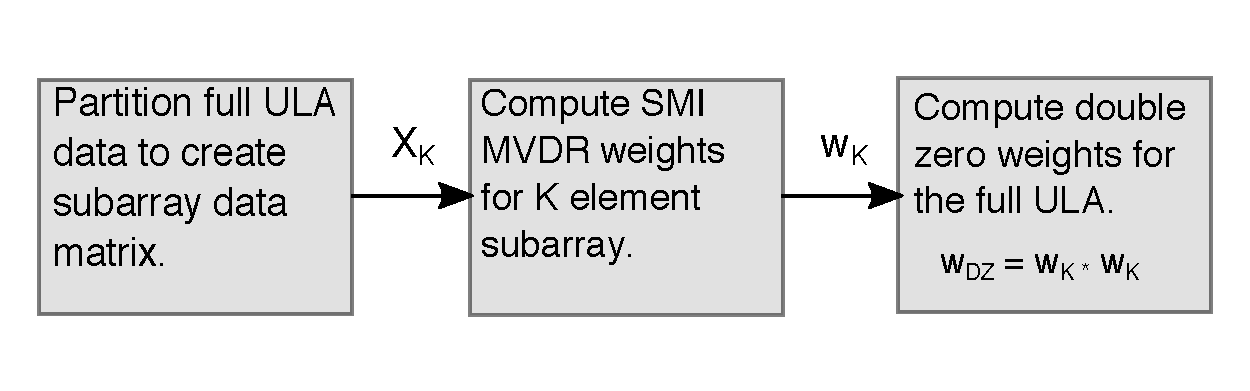
\includegraphics[width=5in]{dz_mvdr_flow.pdf}%
    \label{fig:flow}}
  \vfil

  \subfloat[] 
  {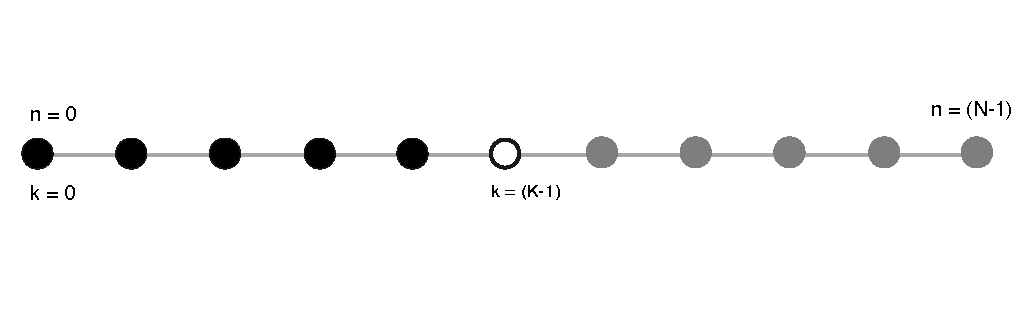
\includegraphics[width=5in]{sub_array.pdf}%
    \label{fig:subarray}}

  \caption{DZ MVDR algorithm (a) flow diagram and (b) two $K$ element
    subarray configuration within the $N$ sensor ULA.}
  \label{fig:dzmvdr}
\end{figure}
% ------------------------------------------------------

The DZ MVDR algorithm involves subarray processing using a $K$ element
subarray. Abraham and Owsley present subarray processing as a
technique to reduce computational overhead for ABFs implemented using
long arrays \cite{abraham89preproc}. The inherent subarray processing
in DZ MVDR ABF also reduces the computational requirement compared to the
standard SMI MVDR ABF implemented on a full ULA saving a factor of 8
in the computation of the SCM inverse. The SCM inversion operation in
\eqref{eq:subarray-wt} takes $\bigO{K^3}$ in contrast to $\bigO{N^3}$
required for the full ULA implementation. Further, the additional
convolution operation in \eqref{eq:wt-convo} takes no more than
$\bigO{K \operatorname{log} K}$. Further, the subarray SCM
($\sampCov_{\rm K}$) is computed using the augmented data matrix with
$2L$ subarray snapshots. The subarray SCM effectively has four times
more snapshots per sensor compared to the standard SCM computed using
the full ULA snapshots. The increase in snapshots to sensor ratio
lowers the bias in the subarray SCM eigenvector estimates which reduces
interferer mismatch \cite{benaych2011eigen, paul2007asymptotics}. The reduction in interferer mismatch enables the DZ MVDR ABF to place deeper notch at the interferer compared to the standard SMI MVDR ABF. 

The computation gain from subarray processing comes at the cost of
reduced spatial degree of freedom (DOF) and widening of the main-lobe
for the DZ MVDR ABF \cite{abraham89preproc}. The DOF is constrained to
about $N/2$, which limits the DZ MVDR ABFs ability to suppress
multiple interferers. Also, the use of $K$ element subarray produces a
main-lobe twice as wide compared to the SMI MVDR ABF using full ULA. A wider main-lobe implies reduced ability of the ABF to resolve two planewaves.

\subsection{Unit circle constrained DZ MVDR ABF}
\label{sec:unit-circle-constr}
As previously seen in Ch.~\ref{ch:mvdr}, the ensemble MVDR beamformer
polynomial zero locations are constrained on the unit circle for
planewave beamforming using a ULA. The DZ MVDR algorithm described
above can be modified to force all the SOZs onto the unit circle
thereby satisfying the unit circle constraint on ensemble case
zeros. In \eqref{eq:subarray-wt}, computing the subarray weights
$\wtK$ as a unit circle (UC) MVDR ABF weights instead of the SMI MVDR
weights produces $K - 1$ zeros $\sampz_{Ki}$ on the unit circle
\cite{tuladhar2015ucmvdr}. The DZ MVDR ABF weight vector $\wtdz$
derived by convolving the subarray UC MVDR weight vector $\wtK$ has
all the SOZs on the unit circle. The unit circle SOZs produce flatter
beampattern nulls and create broader notches in the interferer
direction as discussed in \ref{sec:array-poly-rep}. However enforcing
the UC constraint comes at a cost of additional computational overhead
of solving for the zeros of $K\nth$ order array polynomial to compute
the subarray UC MVDR ABF weights \cite{tuladhar2015ucmvdr}.

% \subsection{Higher-order-zero MVDR }
% \label{sec:higher-order-zero}
% Extending DZ MVDR to higher-order zero implementation for wider nulls.


%%% Local Variables:
%%% mode: latex
%%% TeX-master: "main"
%%% End:
  % algorithm description
\section{Simulation Results}
\label{sec:results}
This section discusses the results of the numerical experiments
evaluating the performance of the DZ MVDR ABF. The experiments are
conducted for two cases: (1) stationary interferers and (2) a moving
interferer. In the stationary interferer cases, the DZ MVDR ABF is
compared with the SMI MVDR and the DL MVDR ABFs. In the moving
interferer case, the DZ MVDR ABF is compared with the CMT MVDR ABF.
In the experiments, all ABFs are implemented using an $N = 31$ element
standard ULA and steered to broadside ($\ulook = 0$). The experiments
assume a passive sonar application where ABFs commonly operate with
barely sufficient snapshots $L = N + 1$ and even $L = 2N$ snapshots
is a relatively snapshot rich case
\cite{cox2002adaptive,baggeroer1999passive}. For all experiments, the
simulated snapshots consists of interferers and unit power white
background noise. No source signal is present in the simulated
snapshot data. All results discussed below are obtained from 3000
trials Monte Carlo experiment.

\subsection{Stationary interferer case}
\label{sec:stat-interf}
Stationary interferers maintain a fixed direction during the snapshot
averaging interval. Two scenarios with stationary interferers are
considered for evaluation of the ABFs. The first scenario has a single
narrowband interferer present at direction $\uinter = 3/N$ with $40$
dB of INR. The second scenario has four discrete narrowband
interferers at directions $\uinter = \{-7/N, ~-3/N, ~3/N, ~7/N \}$
with $\{30, ~20, ~20, ~30 \}$ dB of INR respectively.

\figurename{}~\ref{fig:pout-ecdf} shows the empirical cumulative
distribution function (ECDF) of the output power from the DZ MVDR ABF
compared with the SMI MVDR, and the DL MVDR ABFs. The left panels show
the ECDF graphs for the snapshot limited case ($L = 32$) and the right
panels show the ECDF graphs for the snapshot sufficient case
($L = 62$). The dotted vertical line in each panel denotes the
ensemble output power ($P_{\rm ens}$) produced by the MVDR beamformer
implemented using the knowledge of the ECM. The ensemble output power
is the ideally possible minimum output power for the experimental
scenario. The output power level corresponding to the ECDF value of
$0.5$ denotes the median output power. The closer the median is to the
dotted vertical line, higher the probability of the ABFs to produce
output power comparable to the ensemble output power. The DL factor
for the DL MVDR ABF is set to match the average WNG between the DL
MVDR ABF and the DZ MVDR ABF in each case.

In all four cases in \figurename{}~\ref{fig:pout-ecdf} the DZ MVDR ABF
exhibits higher probability of producing lower output power compared
to the SMI MVDR and the DL MVDR ABF, over the observed output power
range. When snapshot limited ($L = 32$), the DZ MVDR median output
power is less than the SMI MVDR ABF median output power by a factor of
ten. When snapshot sufficient ($L = 62$) the DZ MVDR median output
power is less than the SMI MVDR ABF median output power approximately
by a factor of $1.5$. The DZ MVDR ABF exhibits the greatest
improvement over the SMI MVDR ABF in the snapshot limited
cases. Moreover, the DZ MVDR ABF achieves consistently lower median
output power independent of the snapshots for both single and multiple
interferer scenarios. In contrast, the SMI MVDR ABF's output is
sensitive to the number of snapshots available.

For all interferer scenarios and snapshot conditions, the ECDF of the
DZ MVDR ABF is comparable with the DL MVDR ABF which has the same average
WNG. Examining the snapshot limited ($L = 32$) case for both single
and multiple interferer scenario the DZ MVDR ABF has lower median
output power than the DL MVDR ABF. The lower output power indicates that
the DZ MVDR ABF suppresses the interferer and noise better than the DL
MVDR ABF. In the snapshot sufficient ($L = 62$) case for both single
and multiple interferer scenario, the DZ MVDR and the DL MVDR ABF have
essentially equal median output power. However the DL MVDR ABF
requires a prior choice of the DL factor whereas the DZ MVDR ABF
achieves same performance without the need to choose a design
parameter.

\begin{figure*}[!hp]
  \centering
  \subfloat[Single interferer, L = 32]  {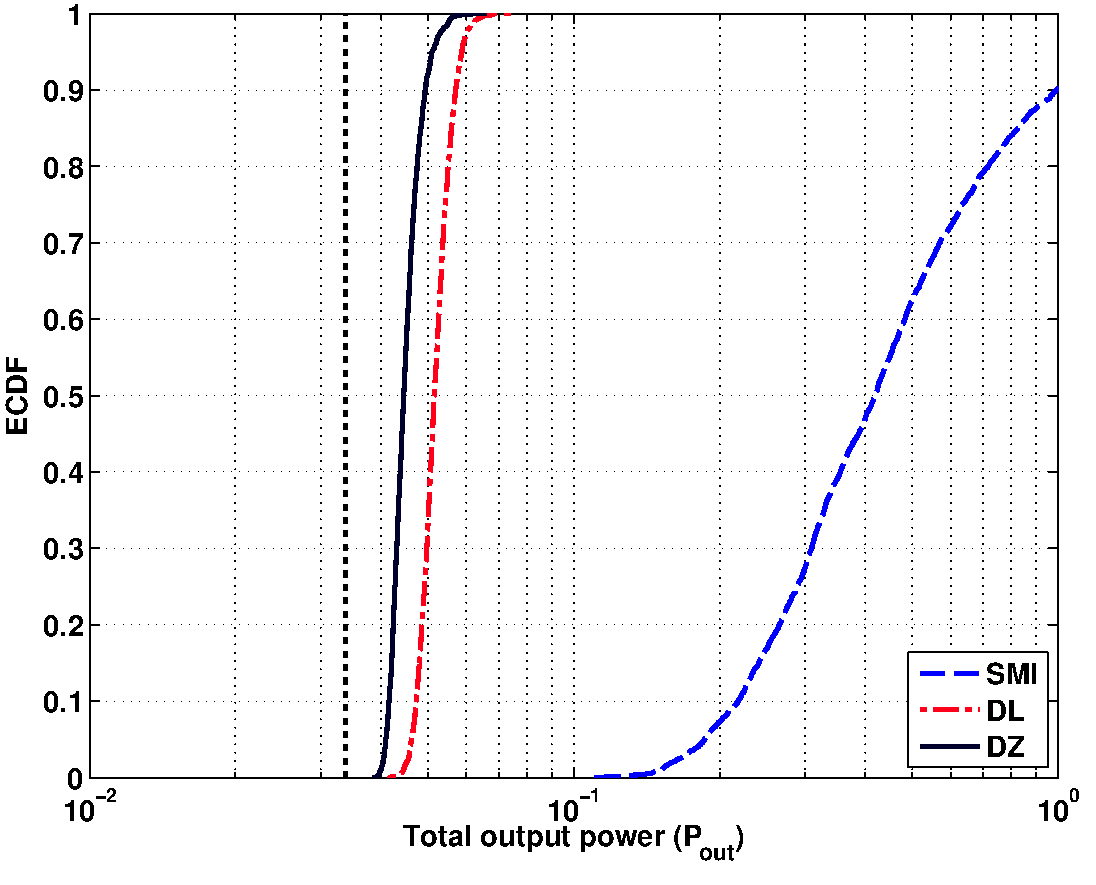
\includegraphics[width=3in]{total_pout_ecdf_single_interf_N31_L32_INR40.pdf}%
    \label{fig:pout-s-L32}}
\subfloat[Single interferer, L = 62]
{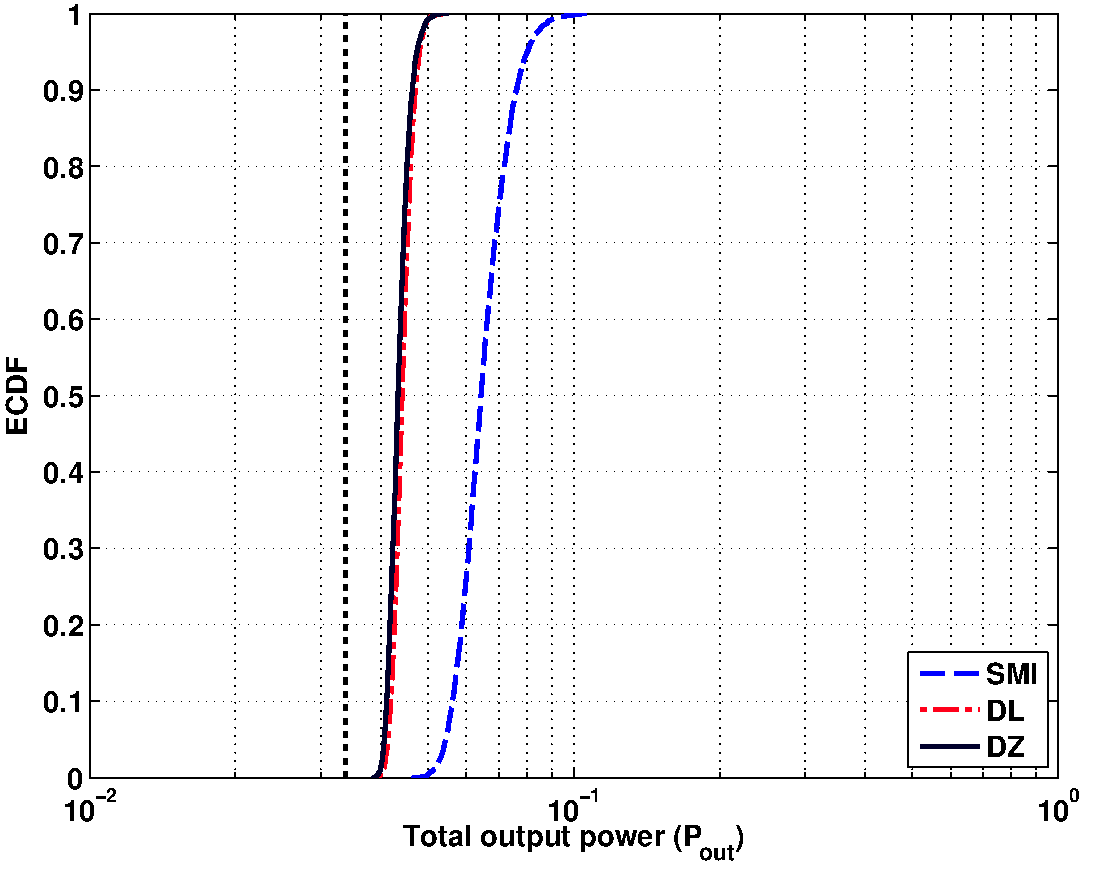
\includegraphics[width=3in]{total_pout_ecdf_single_interf_N31_L62_INR40.pdf}%
    \label{fig:pout-s-L62}}

  \subfloat[Multiple interferers, L = 32]
  {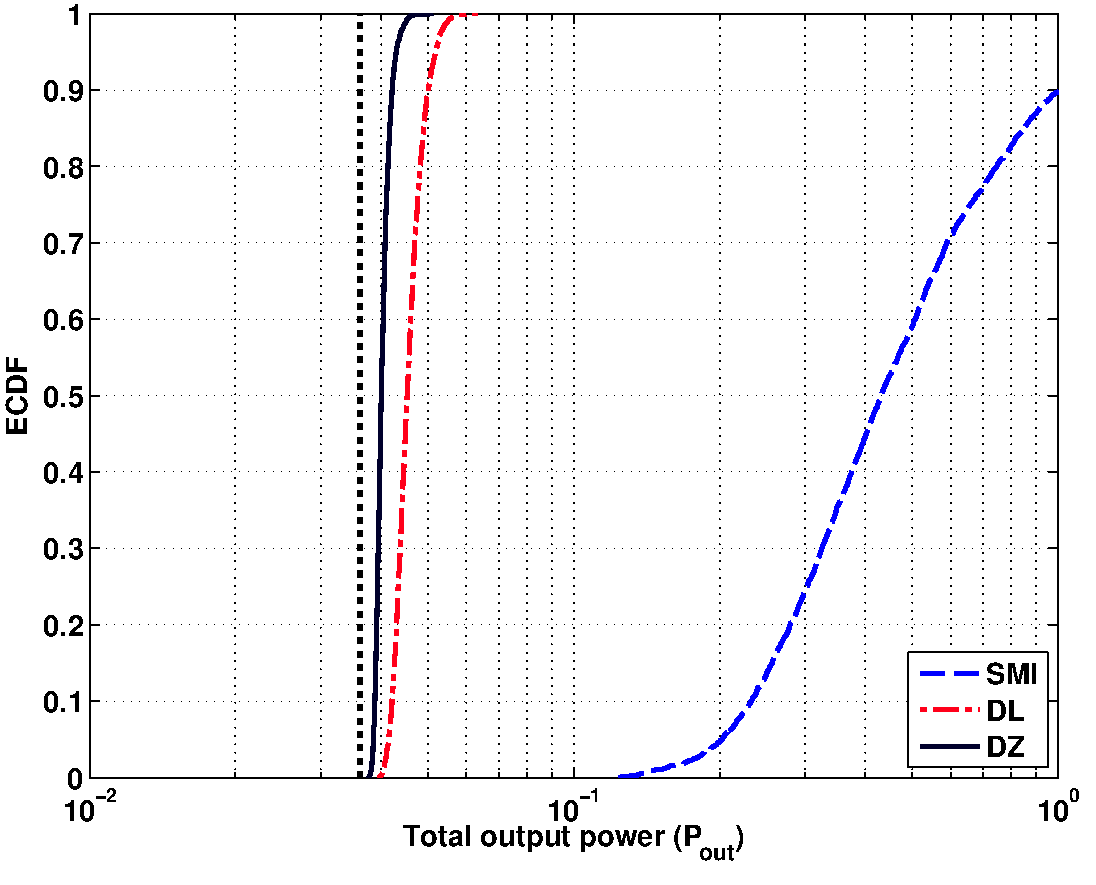
\includegraphics[width=3in]{total_pout_ecdf_multi_interf_N31_L32.pdf}%
    \label{fig:pout-m-L32}}
  \subfloat[Multiple interferers, L = 62]
  {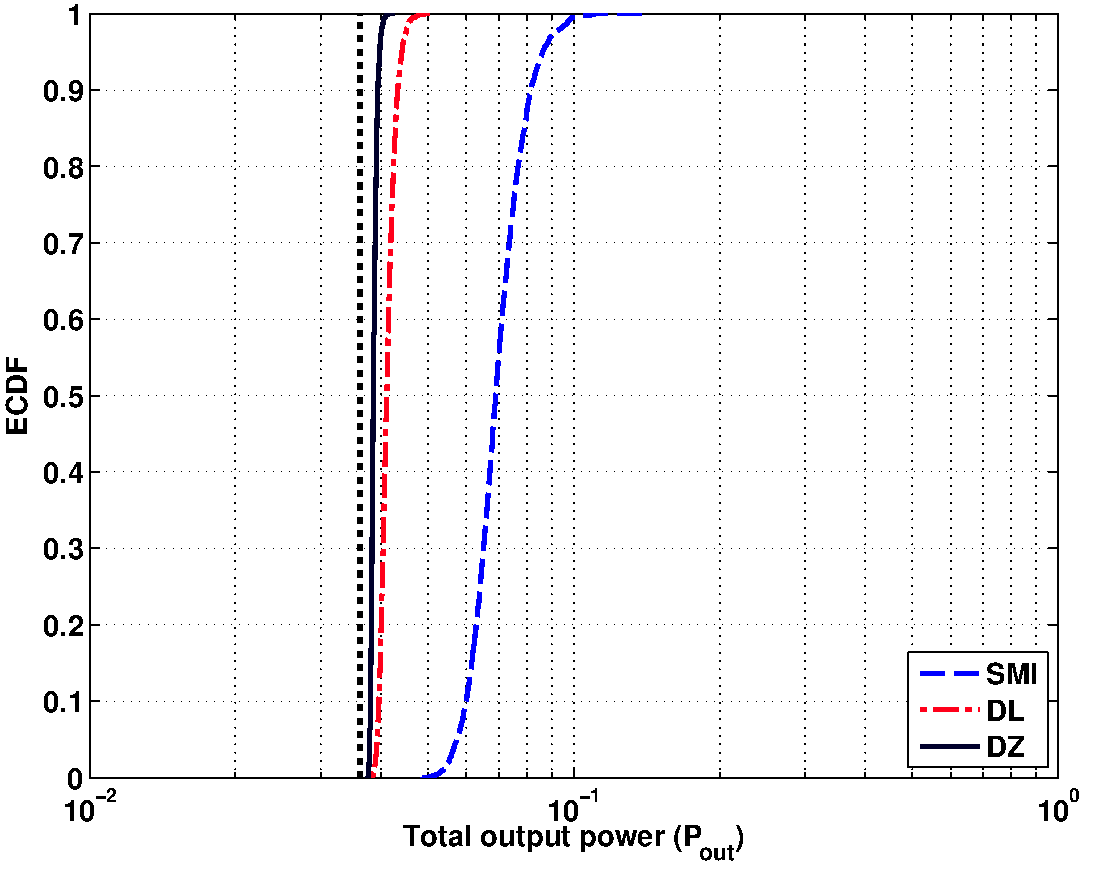
\includegraphics[width=3in]{total_pout_ecdf_multi_interf_N31_L62.pdf}%
    \label{fig:pout-m-L62}}
  \caption{Output power ECDF for the SMI MVDR, DL MVDR and the DZ MVDR
    ABFs using an $N = 31$ element ULA. The vertical dotted line
    denotes the ensemble MVDR output power level. The DZ MVDR ABF has
    higher probability of producing lower output power than the SMI
    MVDR and the DL MVDR ABFs.}
  \label{fig:pout-ecdf}
\end{figure*}

\figurename{}~\ref{fig:ecdf-dz-dzuc} compares output power of the DZ
MVDR ABF and the UC constrained DZ MVDR ABF. The left panel shows the
single interferer scenario while the right panel shows the multiple
interferers scenario in a snapshot limited case ($L = 32$). Comparison
shows that in both scenarios, the DZ MVDR and the UC constrained DZ
MVDR have essentially the same ECDF. The UC constraint yields only a
minimal improvement over the DZ MVDR ABF. Thus, zero doubling in the
DZ MVDR ABF is contributing to most of the gain over SMI MVDR
ABF. Moreover implementing the UC constrained DZ MVDR ABF only
introduces computational overhead as discussed in
Sec.~\ref{sec:unit-circle-constr}. Hence UC constrained DZ MVDR ABF
does not improve performance sufficiently to justify the additional
computational cost of solving for the roots of the $K = 16\nth$ order
array polynomial required for combining the UC and the DZ
algorithms. Also in both interferer scenarios, the DZ MVDR ABF has
lower median output power compared to the standard UC MVDR ABF for a
far smaller computational cost \cite{tuladhar2015ucmvdr}.

\begin{figure}[!ht]
\centering
\subfloat[Single interferer]{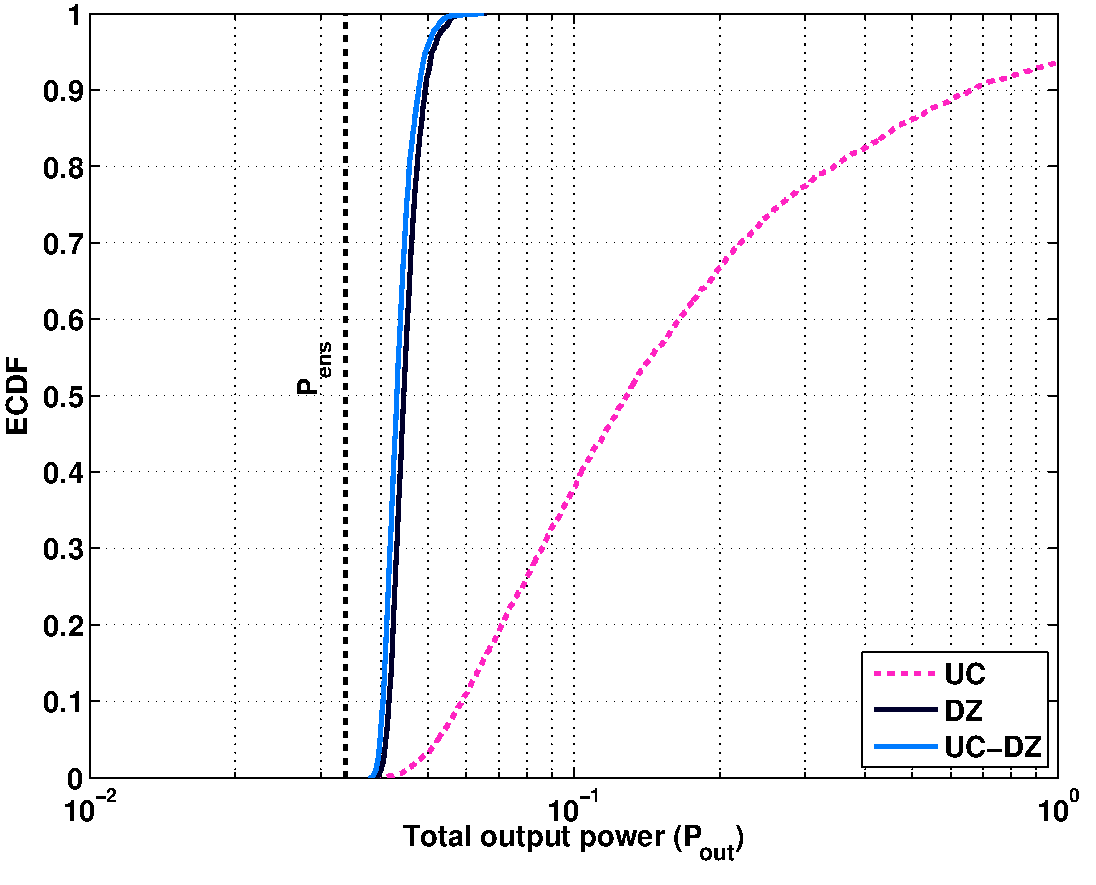
\includegraphics[width=3in]{dz_ucdz_ecdf_comp_single_interf.pdf}}
\subfloat[Multiple interferers]{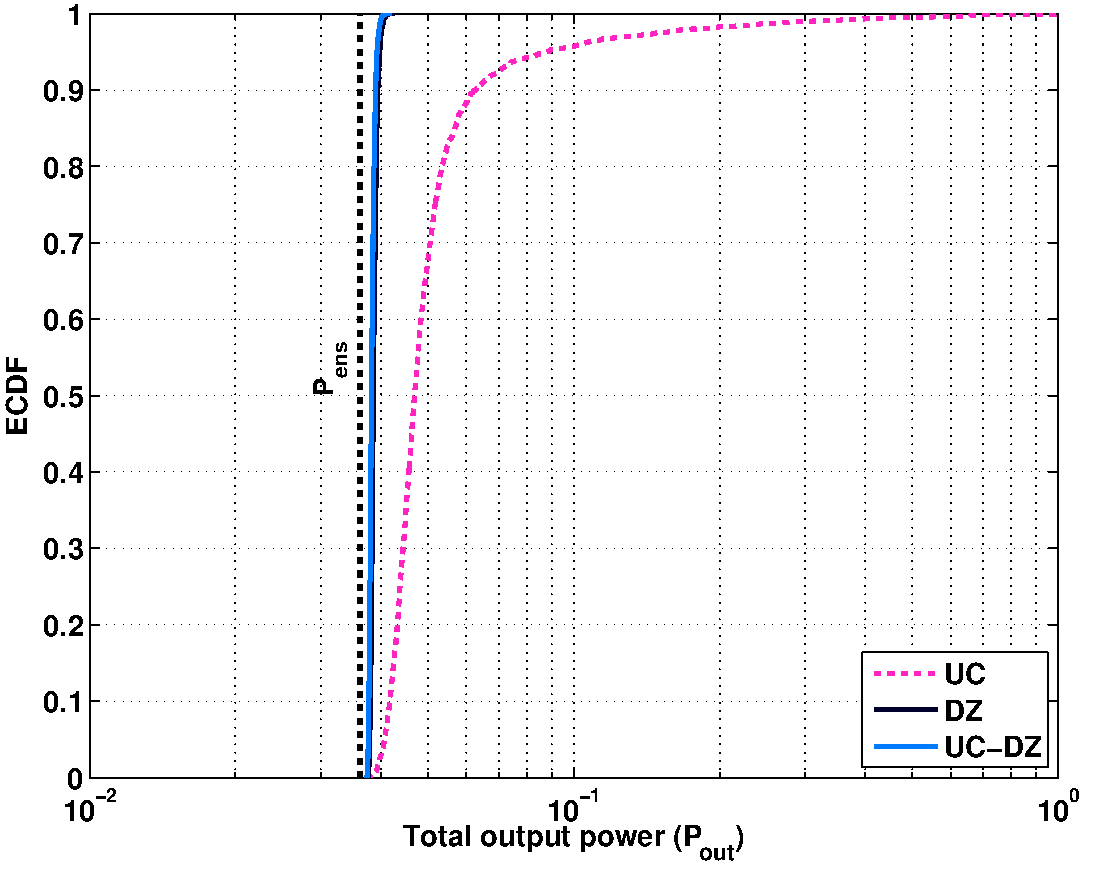
\includegraphics[width=3in]{dz_ucdz_ecdf_comp_multi_interf.pdf}}

\caption{Output power ECDF for the DZ MVDR, the unit circle (UC)
  constrained DZ MVDR and the UC MVDR ABFs using an $N = 31$ element ULA
  and $L = 32$ snapshots. The UC constraint yields only a minimal gain
  over the DZ MVDR ABF.}
\label{fig:ecdf-dz-dzuc}
\end{figure}

% Multi interferer case: dz_ucdz_ecdf_comp_multi_interf

% THIS CAN GO INTO DISSERTATION
% % Mean var result discussion
% \figurename{}~\ref{fig:pout-mean-var-plots} compares the mean (solid) and
% variance (dashed) of the output power for the SMI MVDR ABF and the DZ MVDR
% ABF for the single interferer scenario, over a range of input INR levels
% from $0$ dB to $40$ dB. The DZ MVDR ABF produces output power with both lower
% mean and lower variance compared to the SMI MVDR ABF. The reduced mean output
% power demonstrates the DZ MVDR ABF's ability to suppress
% interferers. The reduced variance on output power suggests the DZ MVDR
% beamformer should achieve better detection performance as well.

% % Mean and var figure
% \begin{figure*}[!t]
%   \centering
%   \subfloat[$L = 32$]
%   {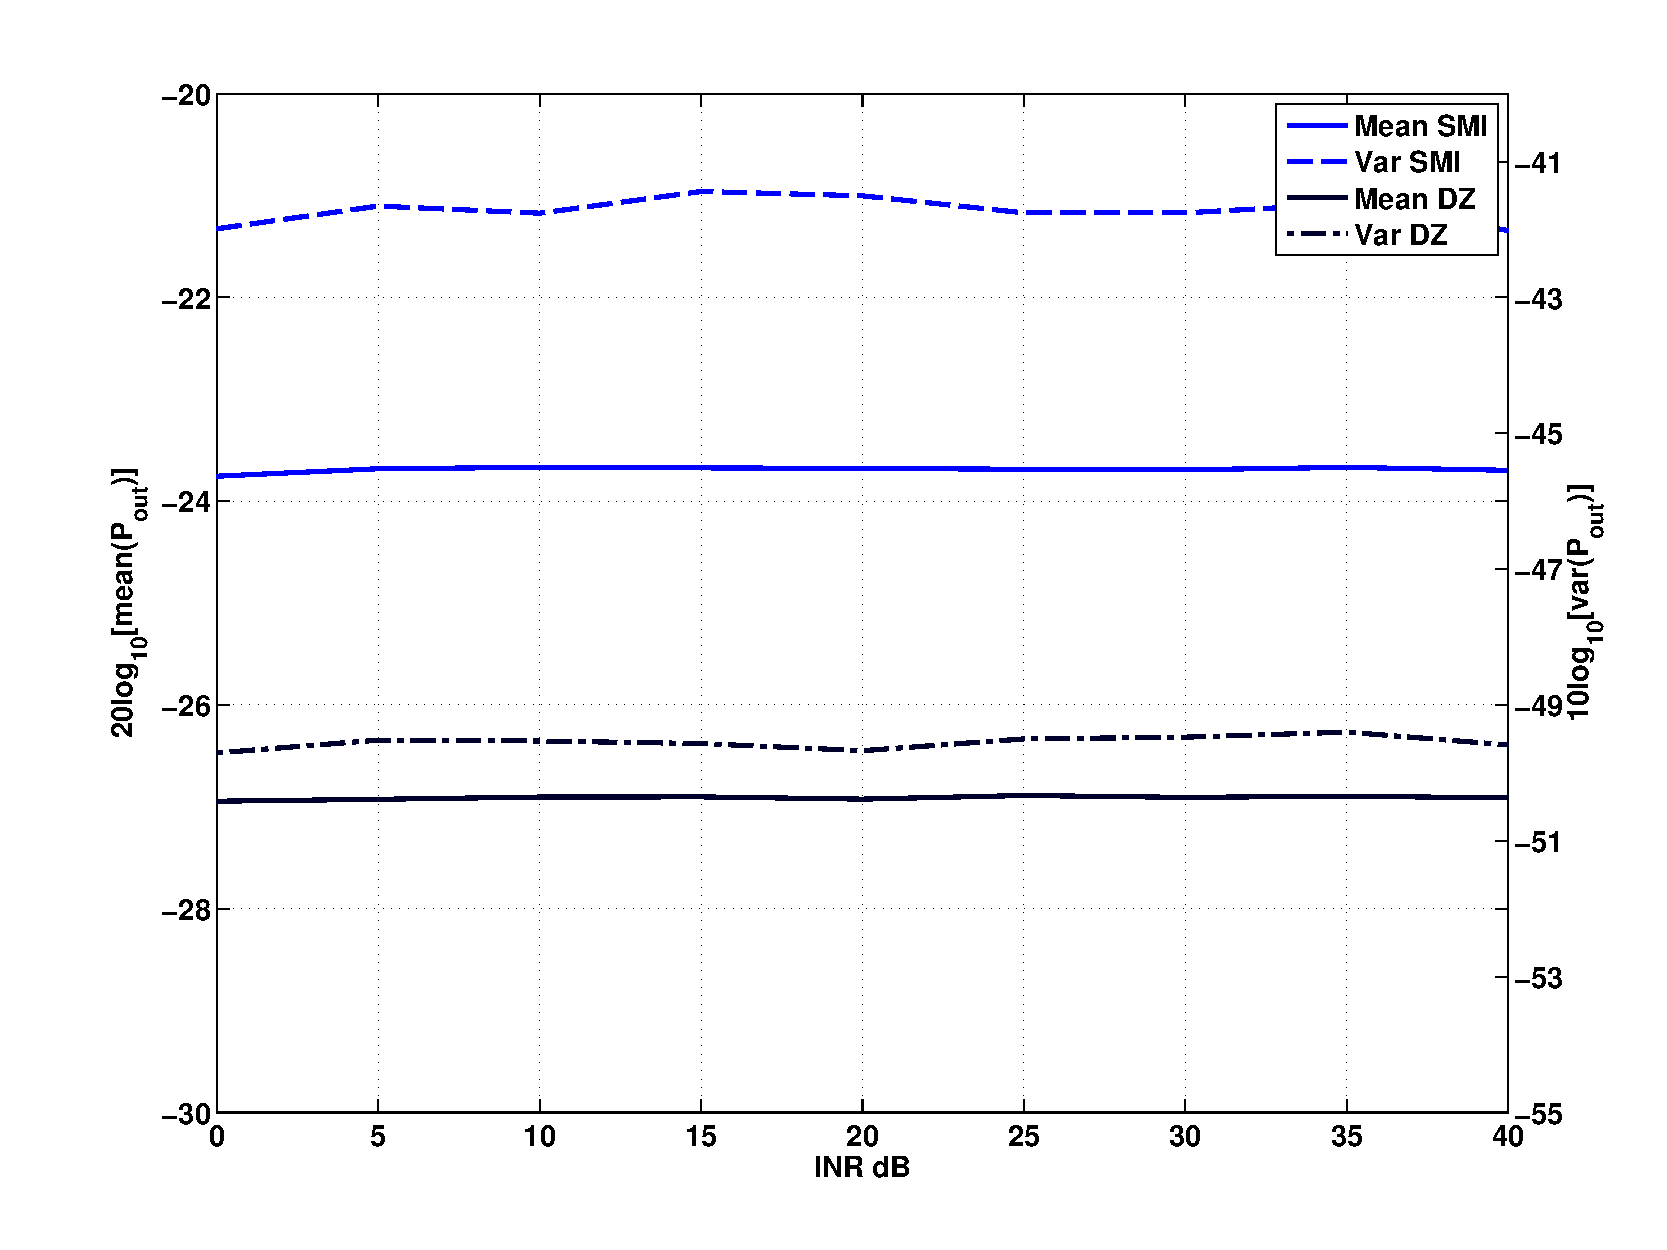
\includegraphics[width=2.8in]{mean_var_Pout_single_interf_N31_L62.pdf}
%     \label{fig:mean-var-single}}
%   \hfil
%   \subfloat[$L = 62$]
%   {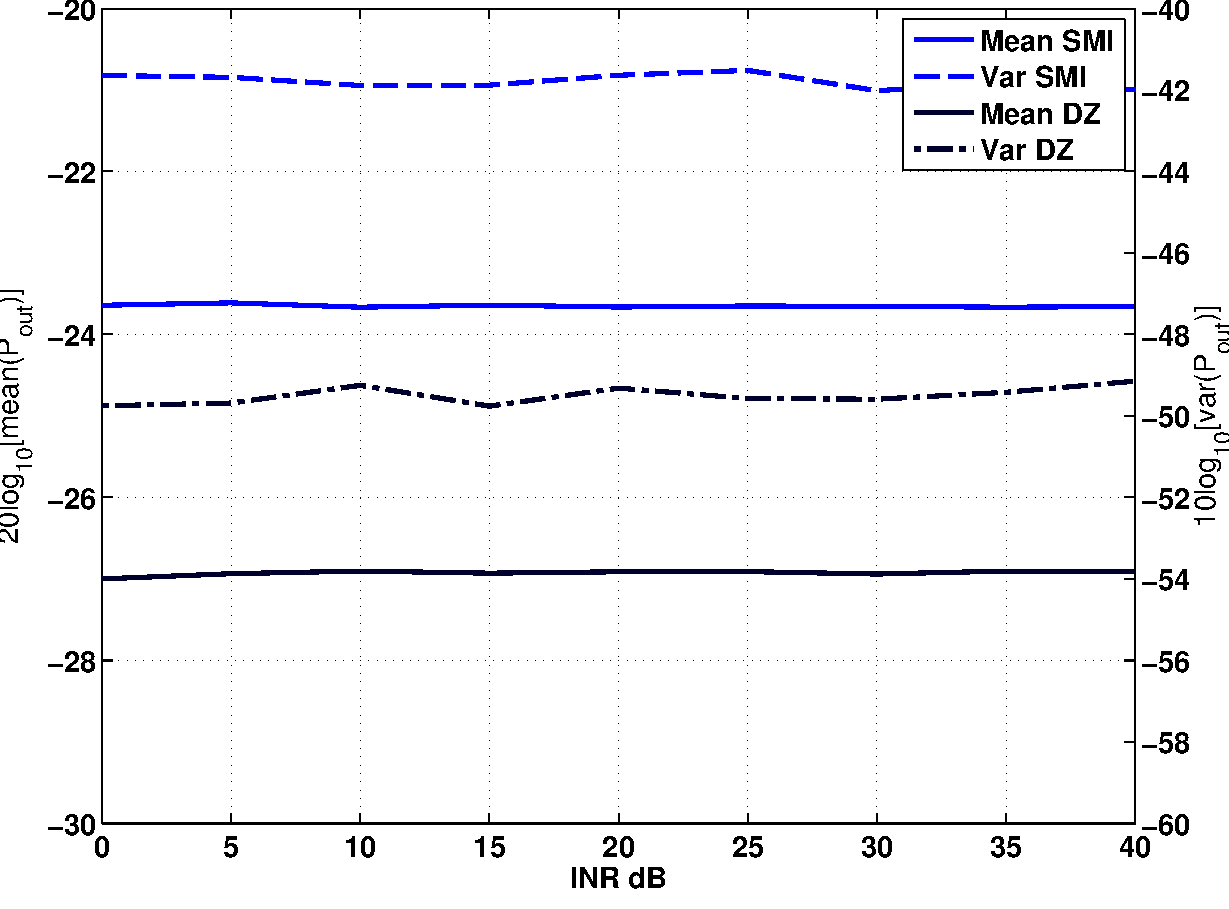
\includegraphics[width=2.8in]{mean_var_Pout_multi_interf_N31_L62.pdf}
%     \label{fig:mean-var-multi}}
%   \caption{Mean and variance of ABF output power over a range of input
%     INR for single interferer case. The DZ MVDR ABF output power has both lower mean and variance
%     compared to the SMI MVDR ABF.}
%   \label{fig:pout-mean-var-plots}
% \end{figure*}

% WNG discussion
\figurename{}~\ref{fig:wng-scatter} shows a scatter plot of the WNG
for the DZ MVDR and the SMI MVDR ABF. The top panel shows single
interferer scenario and the bottom panel shows the multiple interferer
scenario. In both plots, dot markers denote the snapshot limited case
($L = 32$) and the asterisk markers denote the snapshot sufficient
case ($L = 62$). Each dot and asterisk plots the WNG of the DZ MVDR
ABF against the WNG of the SMI MVDR ABF for one realization in the
Monte Carlo experiment. The optimal WNG for the experiment is $N = 31$
and the top right corner of the panel corresponds to the optimal WNG
for both ABFs \cite{vtree2002oap}. For all interferer scenarios and
snapshot conditions examined, the DZ MVDR ABF has better WNG than the
SMI MVDR ABF for almost every experimental trial. The DZ MVDR ABF
achieves consistently high WNG independent of the number of snapshots
for both the single and multiple interferer scenarios. In contrast,
the SMI MVDR ABF's WNG is very sensitive to the number of snapshots
available.  From the scatter plots, the DZ MVDR ABF exhibits higher
WNG on average compared to the SMI MVDR ABF. In addition to improving
the DZ MVDR ABF's ability to reject white background noise, the
improved WNG also indicates improved robustness against parameter
mismatch \cite{Gilbert1955}.

\begin{figure*}[!hp]
\centering
\subfloat[Single interferer]{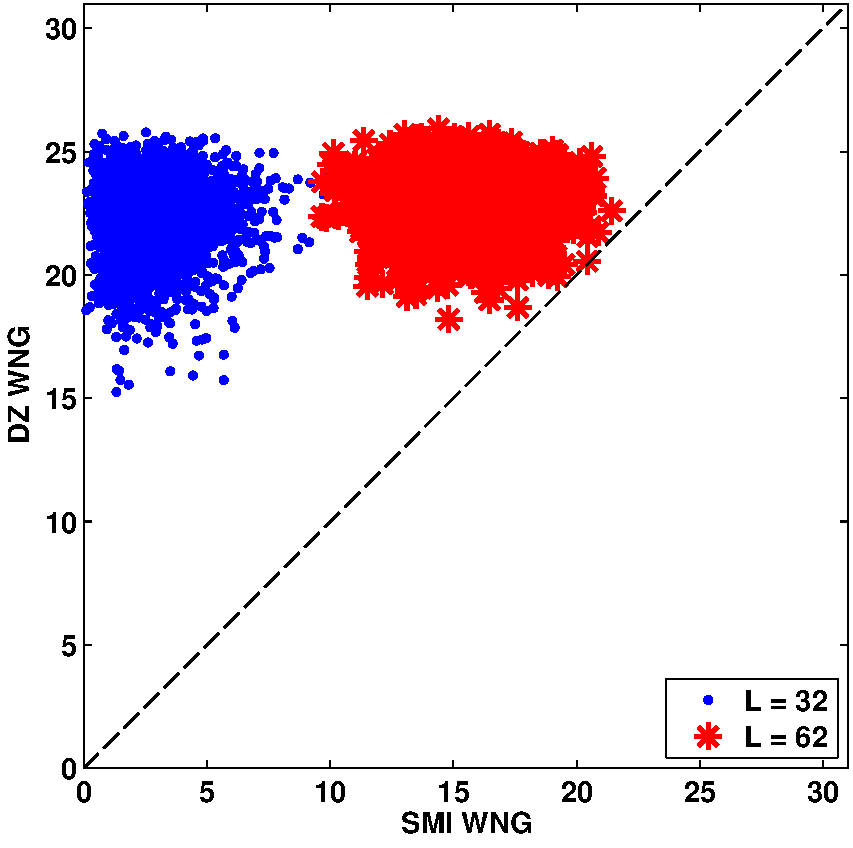
\includegraphics[width=3in]{wng_scatter_composite_single_N31.pdf}
%\subfloat[L = 32]{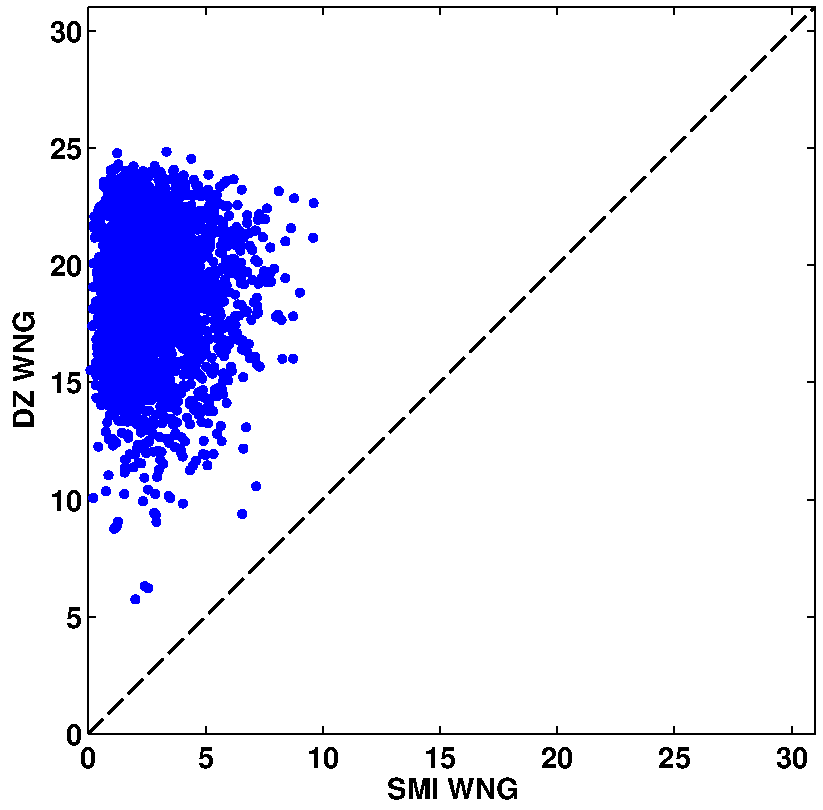
\includegraphics[width=2.5in]{wng_single_interf_N31_L32_INR40.pdf}
\label{fig:wng-s-L32}}

\subfloat[Multiple interferer]{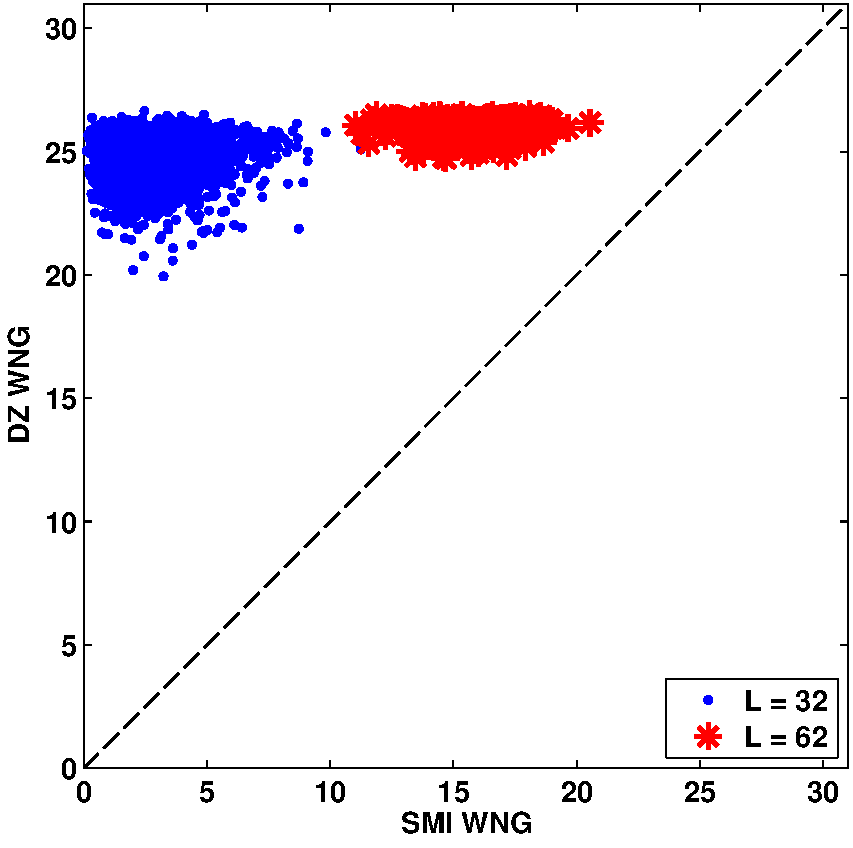
\includegraphics[width=3in]{wng_scatter_composite_multi_N31.pdf}
%\subfloat[L = 62]{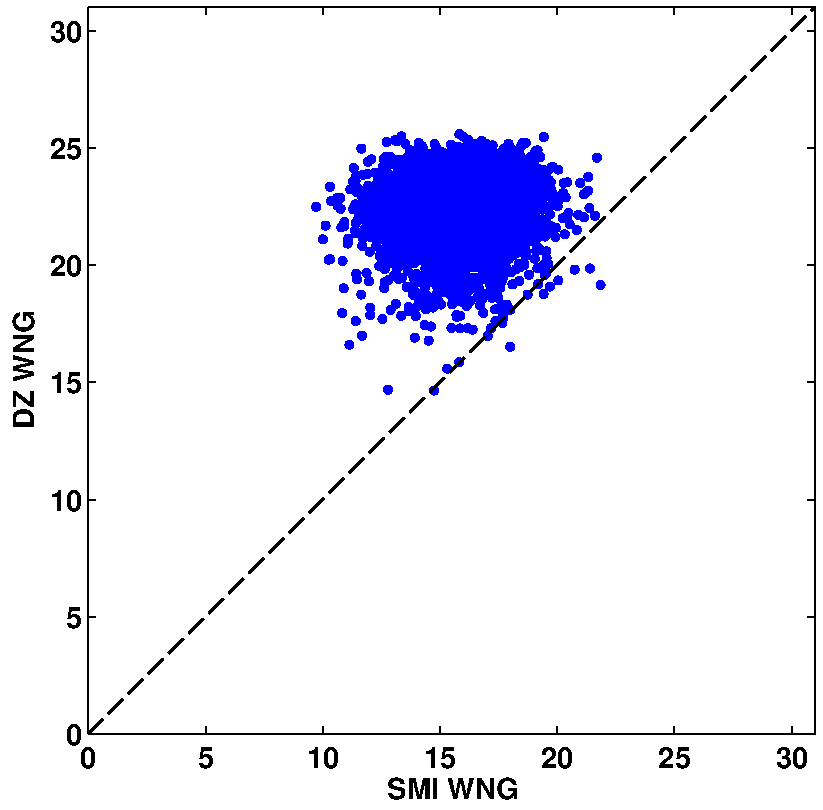
\includegraphics[width=2.5in]{wng_single_interf_N31_L62_INR40.pdf}
\label{fig:wng-s-L62}}
\caption{WNG scatter plot comparing the DZ MVDR and the SMI MVDR ABFs
  using an $N = 31$ element ULA. On average, the DZ MVDR ABF has a
  higher WNG.}
\label{fig:wng-scatter}
\end{figure*}

% Output vs snapshot
\figurename{}~\ref{fig:pout-snapshot} compares the mean output power
between the DZ MVDR, the SMI MVDR, and the DL MVDR ABFs for
implementations using $L = [32, 48, 62]$ snapshots. The top panel
shows the single interferer scenario and the bottom panel shows the
multiple interferer scenario. In both panels, the solid horizontal
line denotes the ensemble MVDR output power. For both interferer
scenarios and all snapshot cases, comparisons show that the DZ MVDR ABF
produces consistently lower mean output power compared to the SMI MVDR
ABF. When snapshot rich ($L = 62$), the DZ MVDR ABF output power is
lower than the SMI MVDR ABF output only by a factor less than two in
both the single and the multiple interferer scenarios. But when
snapshot limited ($L = 32$) the DZ MVDR ABF mean output power is lower
than the SMI MVDR ABF mean output power by a factor more than ten. As
mentioned previously, the decrease in the number of snapshots results
in an increased interferer direction mismatch. The mismatch leads to the
loss of interferer suppression for the SMI MVDR ABF and produces
higher output power. At the same time, the DZ MVDR ABF with its
broader notches is robust against the interferer direction
mismatch. The broader notches consistently suppress the interferers to
produce lower mean output power compared to the SMI MVDR ABF.

In the experiment, for both interferer scenarios and each snapshot
case, the DL factor for the DL MVDR ABF is chosen to match the average
WNG between the DL MVDR and the DZ MVDR ABFs. Hence the two ABFs have
comparable white noise power suppression. In
\figurename{}~\ref{fig:pout-snapshot}, comparisons between the DZ MVDR
and the DL MVDR ABFs shows that they have essentially same output
power performance for all cases in both interferer scenarios. This
implies that the output power is dominated by white noise contribution
and the interferer power contribution is negligible. Both the DZ MVDR
and the DL MVDR ABFs suppress the interferer power significantly
better compared to the SMI MVDR ABF. However, the approach used to
choose WNG in the experiment is not realistic as it requires
iteratively solving for the DL factor to match the average WNGs. In
practice the DL MVDR ABF still requires choosing a DL factor, while
the DZ MVDR ABF does not require setting a design parameter prior to
implementation. On the other hand, the DL MVDR ABF can in principle
handle more than $N/2$ interferers, while the DZ MVDR ABF is limited
to to about $N/2$ interferers due to the subarray approach
constraining the number of degrees of freedom.

\begin{figure*}[!hp]
\centering
\subfloat[Single interferer]{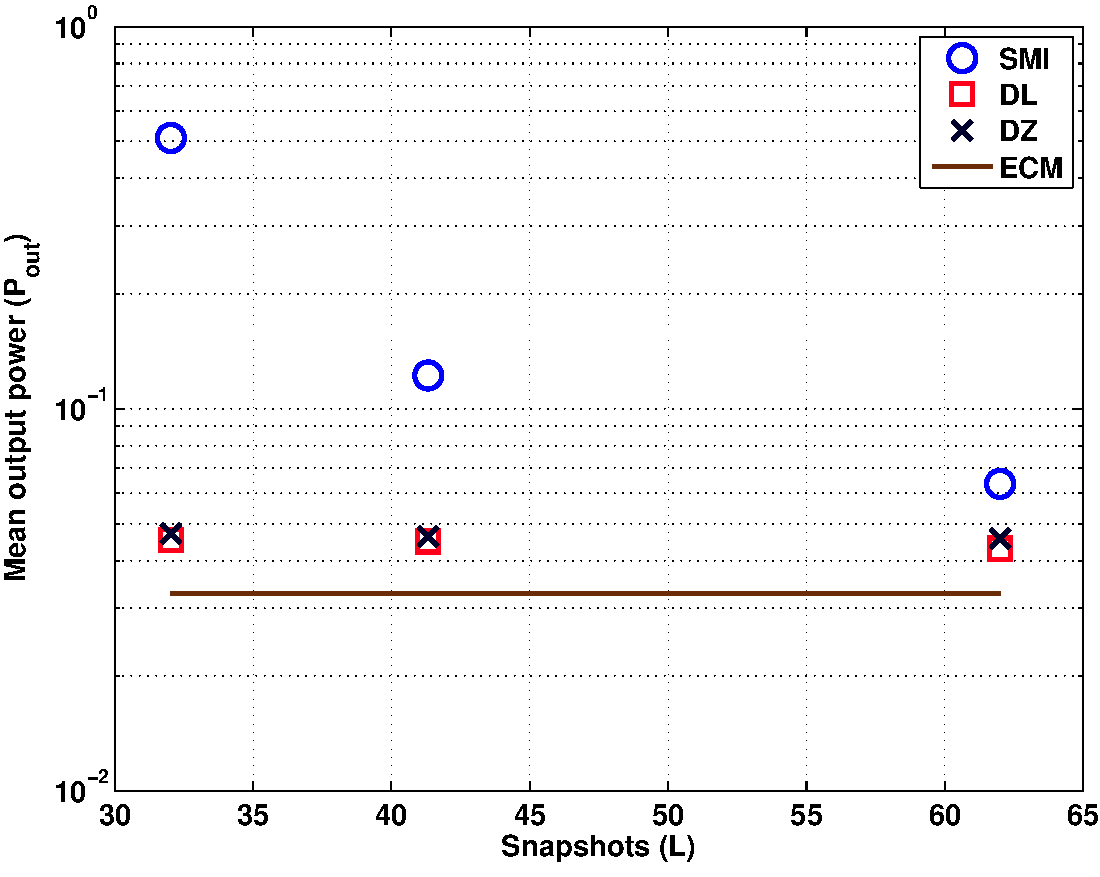
\includegraphics[width=3.5in]{pout_snapshot_N31_single.pdf}
\label{fig:pout-snapshot-L32}}
\hfil
\subfloat[Multiple interferers]{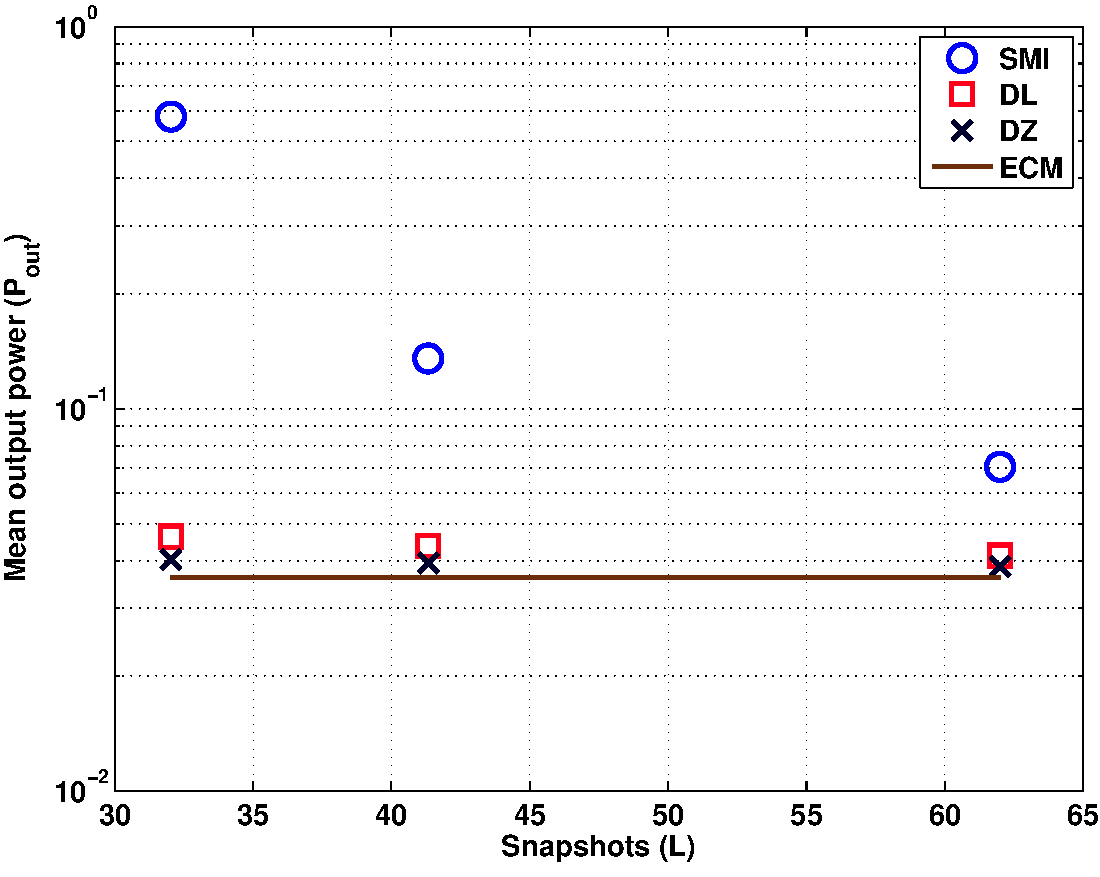
\includegraphics[width=3.5in]{pout_snapshot_N31_multi.pdf}
\label{fig:pout-snapshot-L62}}
\caption{Mean output power from ABFs using different number of
  snapshots for single and multiple interferer cases. The DZ MVDR ABF
  exhibits significant gain over the SMI MVDR ABF in suppressing
  output power when snapshot limited. The DZ MVDR ABF has a mean output
  power comparable with the DL MVDR ABF.}
\label{fig:pout-snapshot}
\end{figure*}

% The inherent subarray processing involved in implementing the DZ MVDR
% ABF widens the main lobe width and limits the degree-of-freedom
% available to suppress interferers to $(N - 1)/2$. But the results
% above indicate that the DZ MVDR ABF is still capable of reducing the 
% output power in presence of multiple interferers compared to the
% traditional SMI MVDR ABF. The consequences of subarray processing is
% further minimized in underwater applications where it is
% common to use long ULAs with hundreds of sensors
% \cite{baggeroer1999passive}. 

\subsection{Moving interferer case} 
\label{sec:moving-interferer}
This section presents results from numerical experiments evaluating
the performance of the ABFs in a moving interferer scenario. The
experiment assumes a scenario containing single spatially moving
interferer in a white background noise similarly to the
example in \cite[Sec. 4]{cox2000mrabf}. The interferer is initially at
direction $u_0 = 5/N$ and moves away from the main lobe at a constant
rate of $\rho_u$ per snapshot. The interferer direction at the
$l^{th}$ snapshot index is $u_l = u_0 + (l-1) \rho_u $ for
$l = 1, \ldots, L$ and $\rep_l = \rep(u_l)$ is the array manifold
vector for the $l\nth$ snapshot. During the snapshot averaging
interval ($l = 1,\ldots, L$), the interferer traverses some fraction
($\mu$) of the ULA resolution width, i.e.,
$\mu = \rho_u (L-1)(N - 1)/2$.

The results compare the output power of the ABFs for
varying interferer velocity cases. In each velocity case, same
number of snapshots $L = 32$ are used to estimate the SCM and compute
the weight vector ($\wthat$) for each ABF. The experiment assumes an
inbred processing approach, where the ABF weights are applied to the
same data used to compute the weights \cite{cox2002adaptive}. Several
other approaches exist for processing data in a non-stationary
environment. However, in order to make a fair comparison between the
ABFs, the experiment uses one consistent approach for all of the ABFs
compared.

In order to evaluate the ABF's output power in the moving interferer
scenario, define a `time averaged' ECM
\begin{align}
  \label{eq:time-avg-ecm}
  \avgCov &= (\interfpow/L)\sum_{l = 1}^{L}\rep_l\rep_l^H +
            \noisepow\eye  \nonumber \\ 
  &= \interfpow\repmat_L\repmat_L\herm + \noisepow\eye,
\end{align}
where $\repmat_L$ is an $N\times L$ matrix of $L$ array manifold
vectors corresponding to the interferer direction $u_l$ at each
snapshot index $l$. The `time averaged' ECM defined in
\eqref{eq:time-avg-ecm} is equivalent to an ECM corresponding to a
scenario containing $L$ independent sources each in the direction $u_l$
with power $\interfpow/L$. This scenario is essentially how the moving
interferer appears to the ULA over the snapshot averaging window
assuming perfect knowledge of the environment. The `time averaged'
ECM captures the interferer motion during the snapshot averaging
window of $l = 1,\ldots, L$. An MVDR beamformer implemented using the
'time averaged' ECM attempts to place a deep notch in each of the $L$
directions ($u_l$).

In the results discussed below, a single realization of the ABF output
power is evaluated as $\pout = \wthat\herm\avgCov\wthat$ where
$\wthat$ is the ABF weight vector. Using the definition of the `time
averaged' ECM in \eqref{eq:time-avg-ecm} the output power is,
\begin{align}
  \label{eq:time-avg-pout}
  \pout &= (\interfpow/L)\wthat\herm\repmat_L\repmat_L\herm\wthat + \noisepow\norm{\wthat}^2 \nonumber \\
&= \pinter + \pnoise,
\end{align}
where $\pinter$ is the output interferer power and $\pnoise$ is the
output noise power. All the results are obtained from a 3000 trial
Monte Carlo experiment assuming the moving interferer with $30$dB INR
and unit power white noise ($\noisepow = 1$). The CMT MVDR ABF is
implemented using the notch width parameter $\cmtW = \resW$.

\figurename{}~\ref{fig:moving-interf-ecdf} compares the output power
ECDF of the DZ MVDR, the CMT MVDR and the SMI MVDR ABFs for the moving
interferer scenario described above. The top panel assumes the
interferer traverses one resolution width during snapshot averaging
($\mu = 1$) and the bottom panel assumes the interferer moves two
resolution widths during snapshot averaging ($\mu = 2$). The dotted
vertical lines on both panels denote the output power from the
ensemble MVDR implemented using the `time averaged' ECM $\Cov_A$. This is the minimum output power achievable using the processing scheme of computing weights from $L$ snapshots. Comparisons
in \figurename{}~\ref{fig:pout-ecdf-mu1}, the case of $\mu = 1$, show
that the DZ MVDR ABF has higher probability of minimizing the output
power compared to the SMI MVDR ABF. The median output power of the DZ
MVDR ABF is more than eight times lower compared to the SMI MVDR ABF.
Also, the ECDF of the DZ MVDR ABF rises faster compared to the ECDF of
the SMI MVDR ABF indicating the output power of the DZ MVDR ABF
exhibits less variability than the output power of the SMI MVDR
ABF. The CMT MVDR ABF also improves performance over the SMI MVDR
ABF. But the DZ MVDR ABF still achieves lower median output power
compared to the CMT MVDR.

Comparisons in \figurename{}~\ref{fig:pout-ecdf-mu2}, the case of
$\mu = 2$, show that the DZ MVDR ABF again has higher probability of
minimizing the output power compared to both the SMI MVDR and the CMT
MVDR ABF. In this case, the interferer is moving at twice the velocity
compared to the case of $\mu = 1$. But the CMT MVDR ABF is still
implemented using the width parameter $\cmtW = 2/N$. The increased
interferer velocity elevates the interferer mismatch problem compared
to the case in \figurename{}~\ref{fig:pout-ecdf-mu1}. Comparing the
two velocity cases, the DZ MVDR ABF median output power increases with
the velocity while the CMT MVDR and the SMI MVDR ABFs have negligible
change in output power.

\begin{figure*}[!hp]
\centering
\subfloat[$\mu = 1$]
{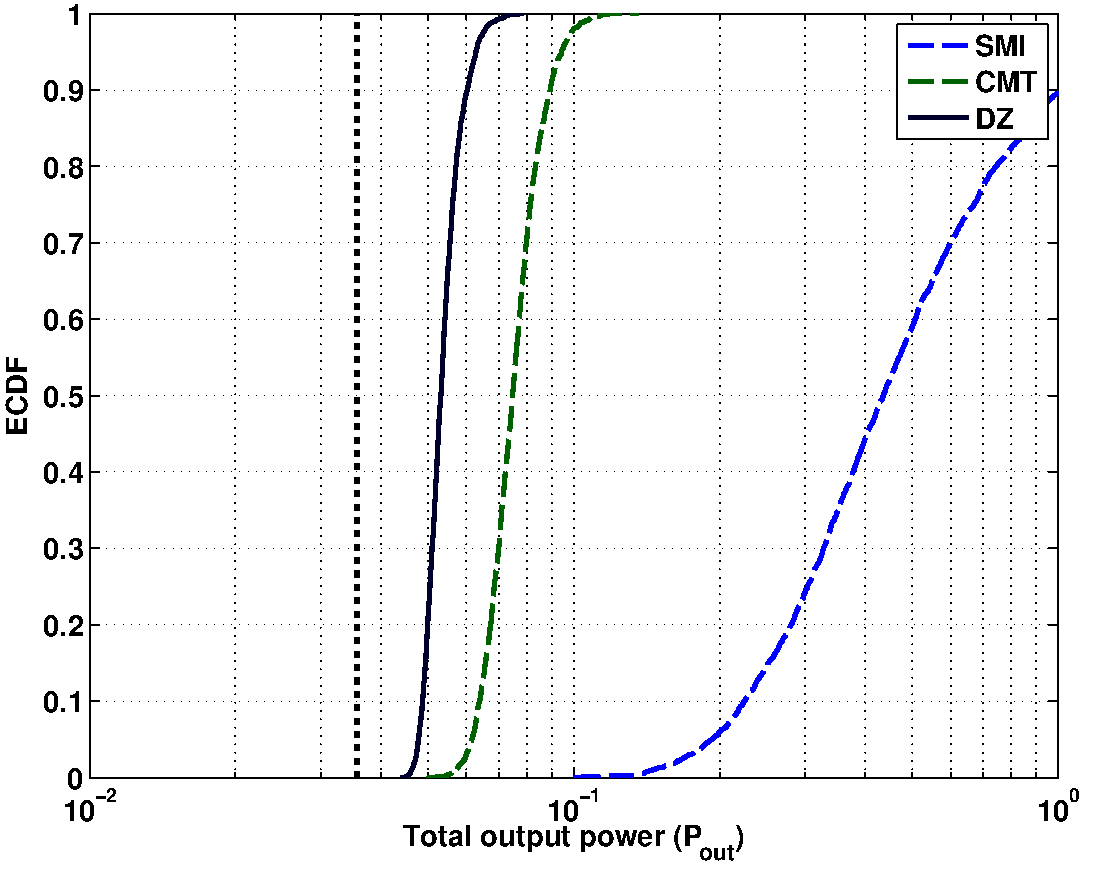
\includegraphics[width=3.5in]{dzmv_moving_interf_pout_ecdf_mu1.pdf}
\label{fig:pout-ecdf-mu1}}

\subfloat[$\mu = 2$]
{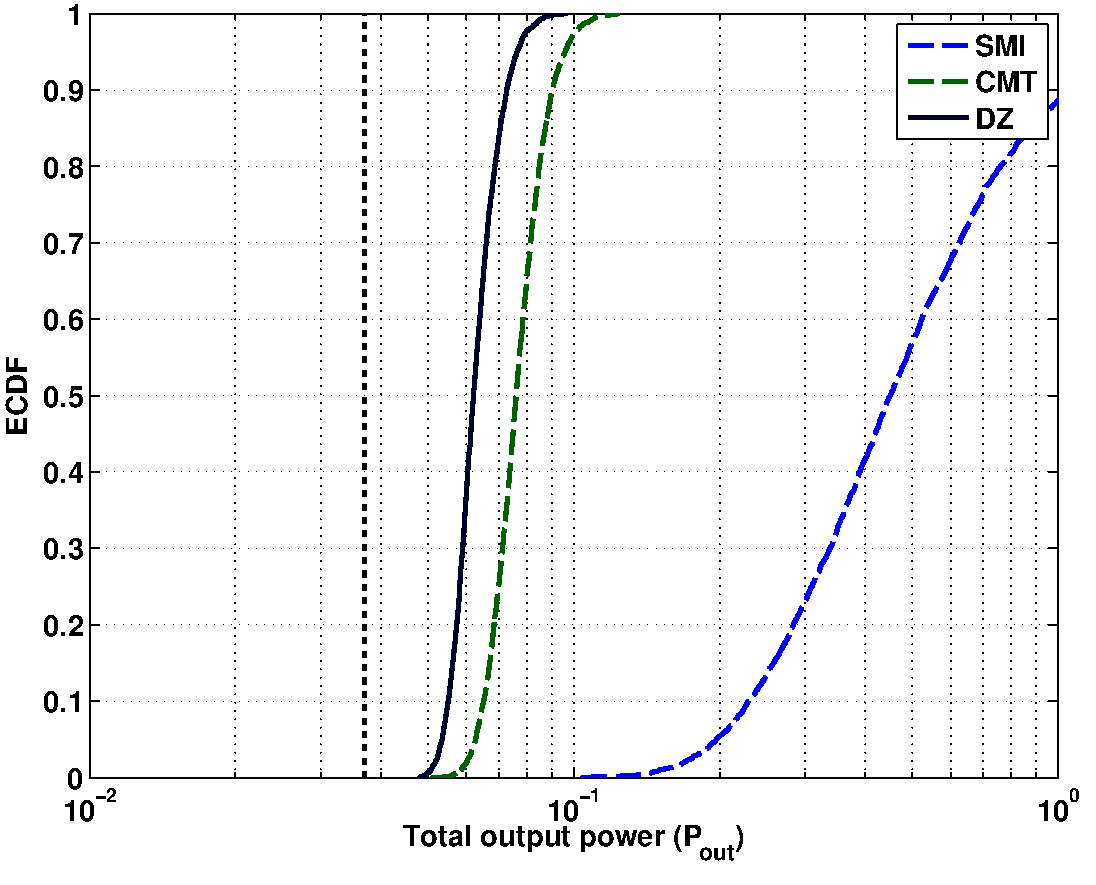
\includegraphics[width=3.5in]{dzmv_moving_interf_pout_ecdf_mu2.pdf}
\label{fig:pout-ecdf-mu2}}
\caption{Total output power ECDF for the DZ MVDR, the CMT MVDR and the
  SMI MVDR ABFs using an $N = 31$ element ULA for two interferer
  velocity cases ($\mu = 1$ and $\mu = 2$). The DZ MVDR ABF has higher
  probability of minimizing output power compared to both the SMI MVDR
  and the CMT MVDR ABF. }
\label{fig:moving-interf-ecdf}
\end{figure*}
\figurename{}~\ref{fig:varying-velocity} compares the outputs from the
DZ MVDR (black diamonds), the CMT MVDR (green squares) and the SMI
MVDR ABF (blue circles) for different interferer velocity cases.  The
top panel shows the interferer contribution to output power
($\pinter$), the middle shows the white noise contribution to output
power ($\pnoise$) and the bottom panel shows the total output power
($\pout$). Since the noise power is assumed to be unity, the noise
contribution to the output power is simply equal to the reciprocal of
the WNG as shown in \eqref{eq:time-avg-pout}.

The experiment evaluates the ABFs for cases when the interferer
traverses $\mu = \{0.5, 1, 2, 3, 4\}$ fraction of resolution width
during $L = 32$ snapshot averaging window. The interferer
contribution, the noise contribution and the total output power is
evaluated as defined in \eqref{eq:time-avg-pout} for each velocity
case. For all velocity cases, the CMT MVDR ABF is implemented with
$\cmtW = 2/N$.

\begin{figure*}[!hp]
\centering
\subfloat[Interferer output power]
{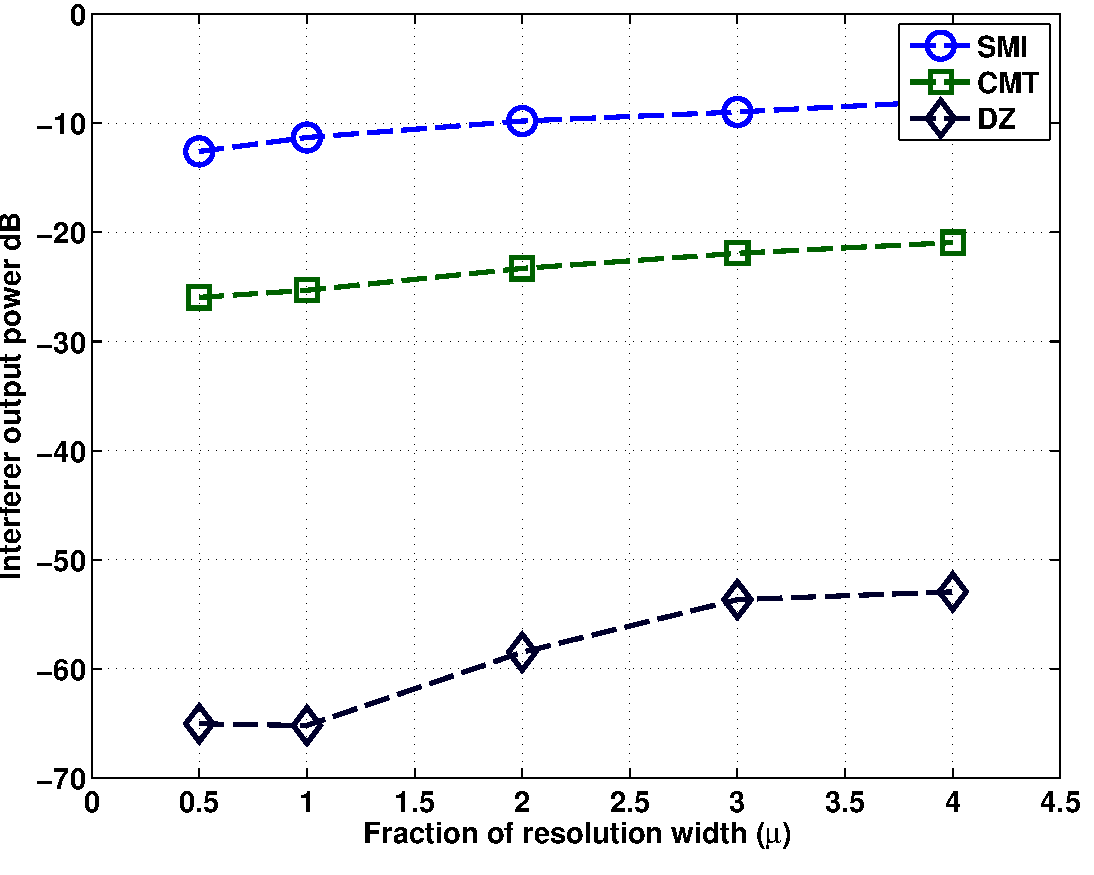
\includegraphics[width=3in]{interf_pout_diff_motion.pdf}\label{fig:interfp-diff-vel}}
\subfloat[WNG]
{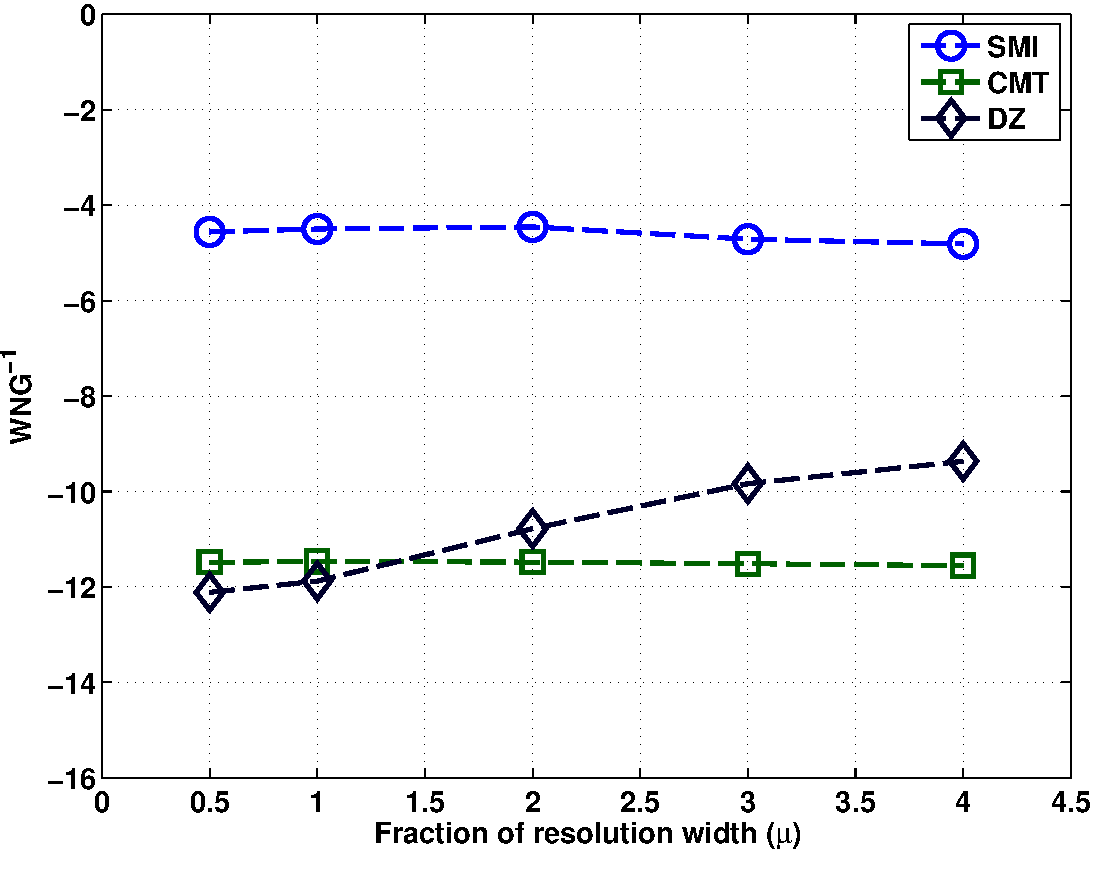
\includegraphics[width=3in]{wng_diff_motion.pdf}\label{fig:wng-diff-vel}}

\subfloat[Total output power]
{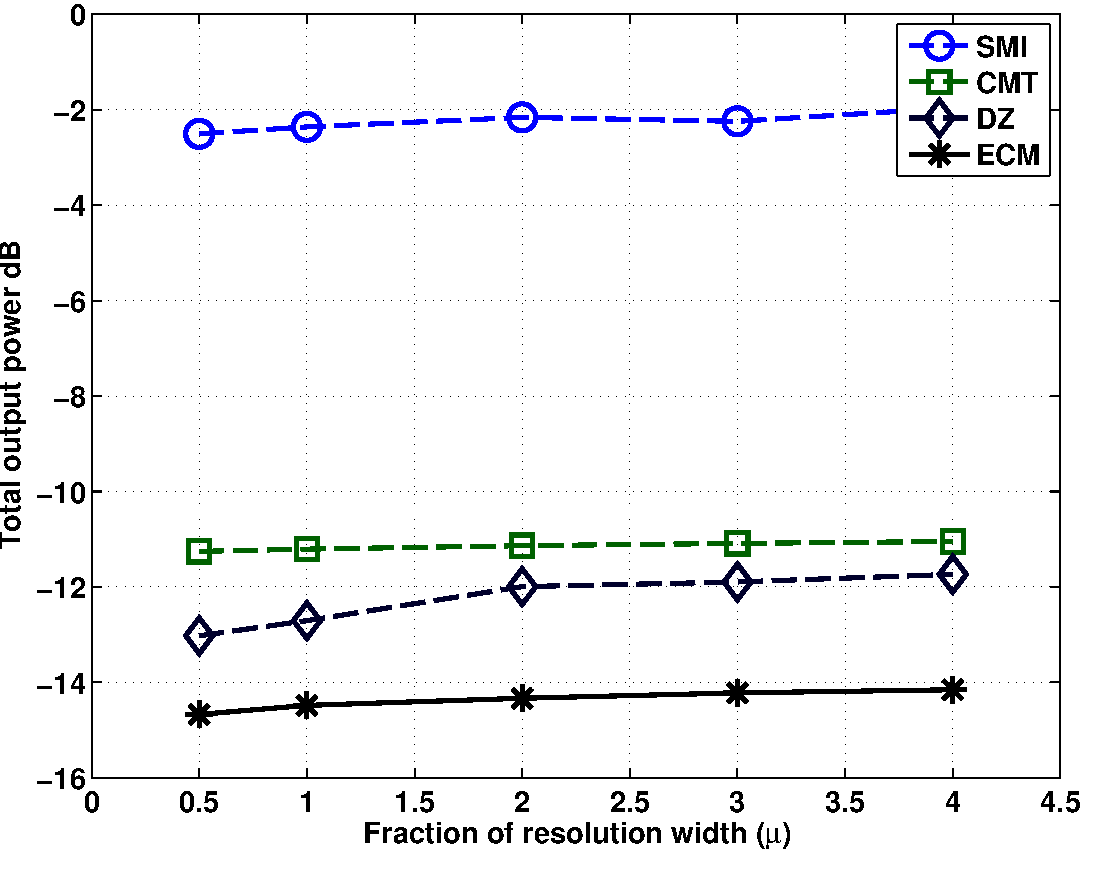
\includegraphics[width=3in]{mean_pout_diff_motion.pdf}\label{fig:outp-diff-vel}}

\caption{Output from the DZ MVDR, the SMI MVDR, and the CMT MVDR ABFs
  using an $N = 31$ element ULA for varying interferer velocity
  cases. The mean output power of the DZ MVDR ABF is about $10$dB
  below the SMI MVDR ABF for all velocity cases. The mean output power
  of the DZ MVDR ABF is comparable with that of the CMT MVDR ABF.}
\label{fig:varying-velocity}
\end{figure*}


\figurename{}~\ref{fig:interfp-diff-vel} compares the mean interferer output power for each ABF at all velocity cases. Comparison shows the DZ MVDR ABF
suppresses interferers significantly better than the SMI MVDR ABF for
all velocity cases. The mean interferer output power for the DZ MVDR
ABF is more than $40$ dB below that of the SMI MVDR ABF in all
velocity cases. Comparatively, the mean interferer output power for
the CMT MVDR ABF is only about $10$ dB below that of the SMI MVDR ABF
in all velocity cases. As mentioned earlier, the DZ MVDR ABF reduces
the estimation bias of interferer eigenvectors as a consequence of
inherent subarray processing. Thus the DZ MVDR ABF is able to create
broader and deeper notch at the interferer and yield better
improvement in interferer suppression compared to the CMT MVDR ABF in
all cases of the experiment.

\figurename{}~\ref{fig:wng-diff-vel} compares the white noise
contribution to output power for each ABF at all velocity cases. The
solid horizontal line denotes the noise output power corresponding to
the optimal WNG of $N = 31$. Comparison shows that the DZ MVDR ABF has
better WNG compared to the SMI MVDR ABF and hence lower output noise
power for all velocity cases. When the interferer motion is limited
within the resolution width ($\mu \leq 1$), the DZ MVDR ABF yields
highest WNG and the lowest output noise power. At higher velocities
($\mu \geq 2$), the DZ MVDR and the CMT MVDR ABF both have comparable
output noise power. 

\figurename{}~\ref{fig:outp-diff-vel} compares the mean total output
power for each ABF at all velocity cases. The black asterisk markers
denote the output power from the ensemble MVDR implemented using the
`time averaged' ECM. The total output power is the combination of
interferer output power and the noise output power. In all velocity
cases, the contribution from the white noise dominates the total
output power for the DZ MVDR and the CMT MVDR ABFs. Both the DZ MVDR
and the CMT MVDR ABF yield significantly lower mean output power
compared to the SMI MVDR ABF in all moving interferer scenarios.
However, the CMT MVDR ABF requires choosing the notch width
parameter while the DZ MVDR ABF does not require setting a design
parameter to produce comparable performance.

\subsection{CMT MVDR ABF with multiple interferers}
\label{sec:cmt-multi-interf}
The CMT MVDR ABF with notch width $\cmtW = 2/(N-1)$ uses three degrees
of freedom (DoF) per interferer to produce broad notch as discussed in
\sect{}~\ref{sec:cmt}. The DZ MVDR ABF by design uses two DoF per
interferer. This section compares the output performance of the CMT
MVDR and the DZ MVDR ABF in case of a multiple interferers scenario.

% To compare the ABFs, consider four interferer directions $\mathbf{\uinter} = \lbrace -7/N,~7/N,~3/N,~-3/N \rbrace$. For all
% four cases, both ABFs are implemented using an $N = 31$ element ULA
% and steered towards broadside ($\ulook = 0$). The CMT MVDR ABF is implemented using notch width $\cmtW = 2/(N - 1$).

\figurename{}~\ref{fig:cmt-output-multi} compares the average output
power from the DZ MVDR (black diamonds) and the CMT MVDR ABF (green
circles) for four cases with different number of interferers
$D = 1\,\text{to}\,4$. The experiments starts with $D = 1$ interferer
at $\uinter = -7/N$ and introduces one additional interferer for each
new case. The direction for additional interferers is chosen
sequentially from the set
$\mathbf{\uinter} = \lbrace 7/N,~3/N,~-3/N \rbrace$ respectively. For
all four cases, both ABFs are implemented using an $N = 11$ element
ULA and steered towards broadside ($\ulook = 0$). The CMT MVDR ABF is
implemented using notch width $\cmtW = 2/(N - 1$). Examining the
output power, the DZ MVDR and the CMT MVDR ABF produce comparable
output for $ D \leq 2$. But for $D > 2$, the CMT MVDR ABF produces
significantly higher output power compared to the DZ MVDR ABF.
\figurename{}~\ref{fig:wng-cmt-multi} compares the inverse of the WNG
of the ABFs.  The inverse of WNG is proportional to the white noise
contribution to output power. When $D > 2$ the white noise
contribution of the CMT MVDR ABF increases significantly. In presence
of multiple interferers, the CMT MVDR ABF fails to suppress output
power as it uses more DoF per interferer compared to the DZ MVDR ABF
as discussed below.

The MVDR ABFs using $N = 11$ element ULA and steered to a fixed look
direction are limited to $N-2 = 9$ DoF for adaptation. When $D = 2$,
the CMT MVDR uses six DoF to suppress interferer and the remaining
DoFs are used for white noise suppression. But when $D = 3$, the CMT
MVDR ABF uses all nine DoF to suppress interferer leaving no DoF for
white noise suppression. This results in loss of WNG for the CMT MVDR
and subsequent increase in white noise contribution to output
power. Moreover when $D = 4$, the CMT MVDR ABF requires more than nine
DoF, which results in failure to suppress interfere and loss of
WNG. As a result the CMT MVDR ABF produces significantly high output
power. In contrast, even when $ D = 4$, the DZ MVDR uses only eight
DoF to suppress interferers. As a result the DZ MVDR ABF consistently
produces lower output power for all four interferer cases.

\begin{figure*}[!hp]
  \centering
  \subfloat[Total output power]{    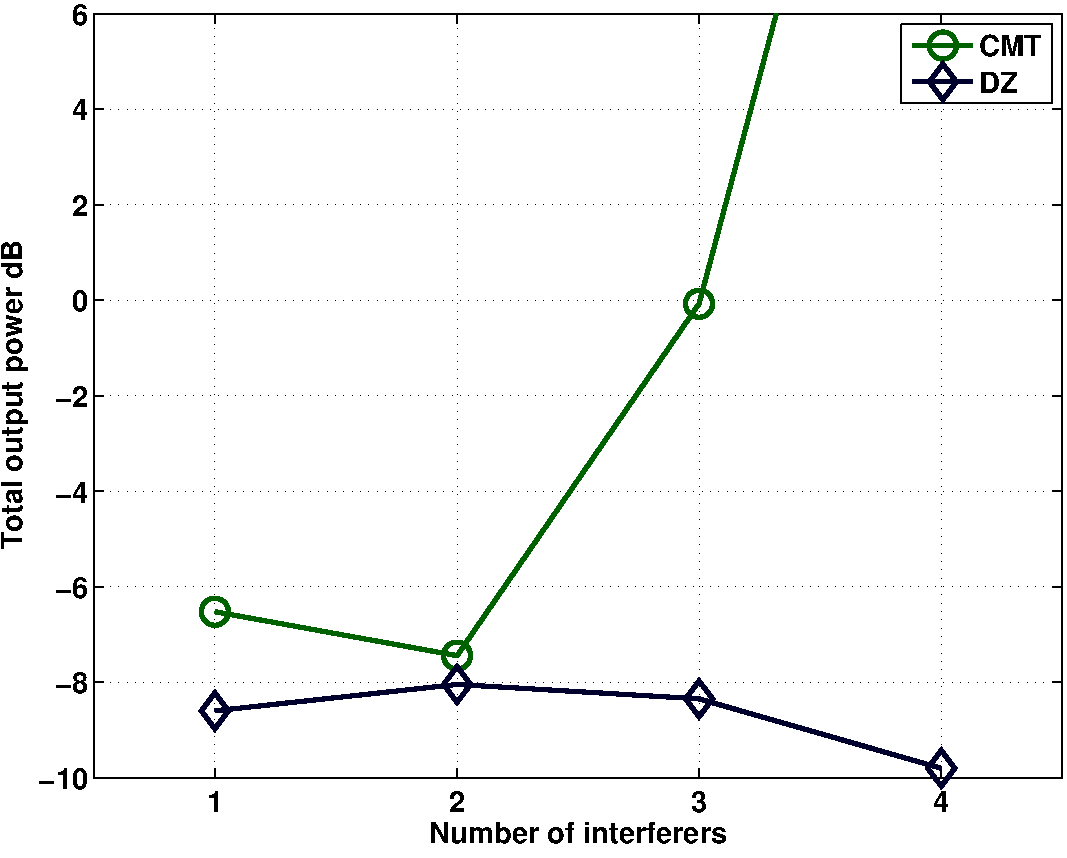
\includegraphics[width=3.5in]{./cmt_multi/dz_vs_cmt_Pout_multi_case2.pdf}
    \label{fig:cmt-output-multi}}

  \subfloat[White noise contribution]{
    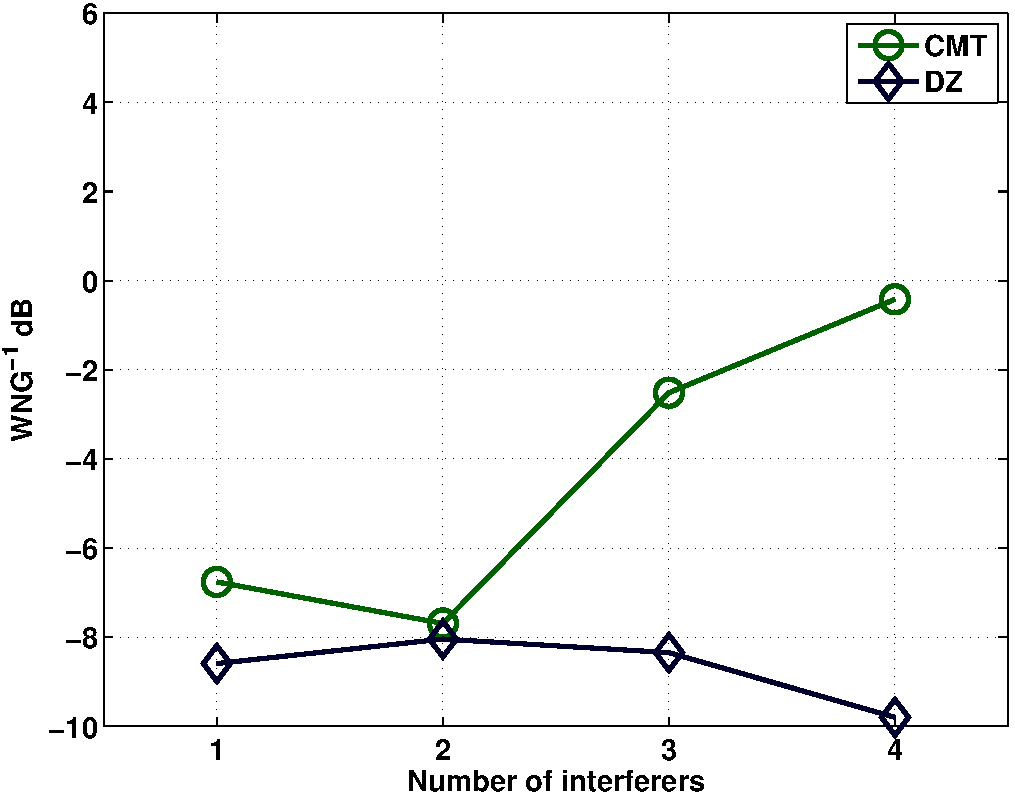
\includegraphics[width=3.5in]{./cmt_multi/dz_vs_cmt_wng_multi_case2.pdf}
    \label{fig:wng-cmt-multi}}
  \caption{Comparison of (a) Output power and (b) white noise
    contribution to output from the DZ MVDR and the CMT MVDR ABFs for
    different number of interferers. Both ABFs are implemented using
    $N = 11$ sensor ULA and steered towards broadside. The CMT MVDR
    uses notch width of $\cmtW = 2/(N-1)$. As the number of
    interferers increases, the CMT MVDR fails to suppress output power
    as it uses more DoF per interferer compared to the DZ MVDR ABF.}  
\end{figure*}

% As previously mentioned, the DZ MVDR ABF has only $(N-1)/2$ degrees of
% freedom (DoF) for interferer suppression. Equivalently the DZ MVDR
% polynomial has only $(N-1)/2$ unique zeros for interferer
% suppression. On the other hand, the CMT MVDR ABF using full ULA has
% $(N - 1$) DoF for interferer suppression. Equivalently the CMT MVDR
% polynomial has $N-1$ zeros for interferer suppression. However, as
% mentioned in \sect{}\ref{sec:cmt}, depending on the notch width, the
% CMT MVDR ABF uses multiple zeros per interferer to produce broad notch
% which reduces the effective DoF available for interferer
% suppression. As the number of interferers increases more zeros are
% used for notch broadening and fewer zeros are available for the white
% noise suppression.

% \figurename{}~\ref{fig:cmt-zeros-multi} shows a representative example
% of DZ MVDR polynomial zeros (black) and the CMT MVDR polynomial zeros
% (green). For simplicity, the example uses $N = 11$ element ULA. The
% dotted radial lines indicated the four interferer directions
% $\mathbf{\uinter} = [-7/N,~7/N,~3/N,~-3/N]$ considered in
% \figurename{}~\ref{fig:cmt-output-multi}. The DZ MVDR ABF places a SOZ
% in the vicinity of each interferer direction to produce broad
% notches. Comparatively, the CMT MVDR ABF places up to three zeros in
% the vicinity of the interferer directions. As a result, all ten of CMT
% MVDR polynomial zeros are used to produce wide notches for merely
% $D = 4$ interferers. The clustering of all zeros in the interferer
% direction yields high sidelobes in between the broad notches. The high
% sidelobes in CMT MVDR beampattern lead to significant loss of the WNG
% and subsequent rise in output power. Since the number of zeros used
% per interferer depends on the choice of the notch width ($\cmtW$), it
% is imperative for the CMT MVDR ABF to use suitable value of
% $\cmtW$. However, the DZ MVDR ABF does not require choosing a design
% parameter and consistently suppresses output power for $D < (N -1)/2$.

% \figurename{}~\ref{fig:cmt-zeros-multi} shows the polynomial zeros for the CMT MVDR (green circles) and the DZ MVDR (black diamonds). The left panel considers the case of $D = 3$ interferers and the right panel considers the case of $D = 4$ interferers. 

% \begin{figure*}[!hp]
%   \centering
%   \subfloat[D = 3]{
%     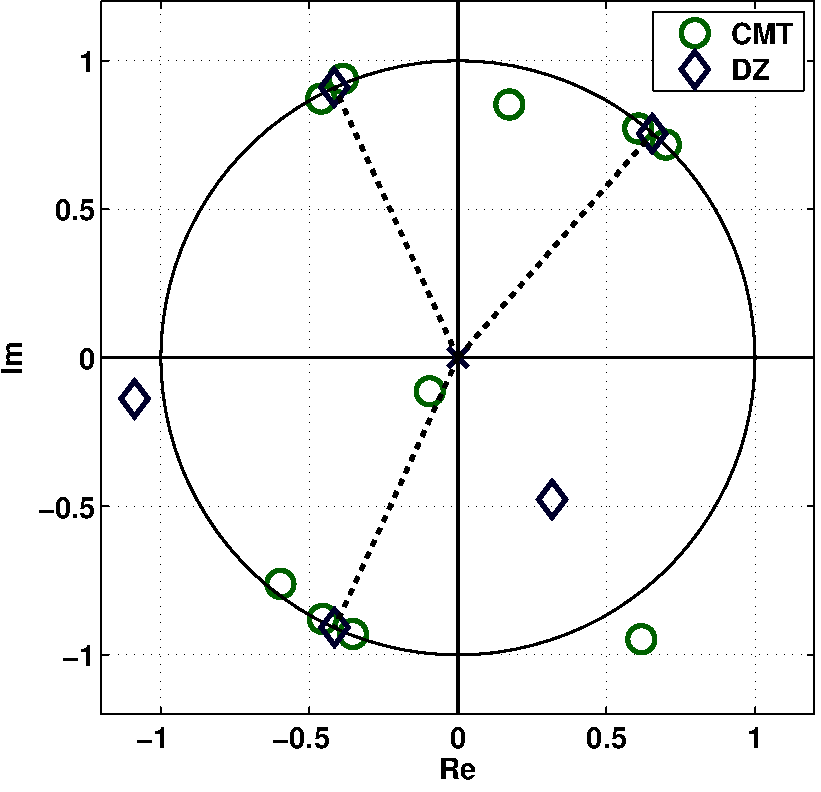
\includegraphics[width=3in]{./cmt_multi/cmt_pzplot_multi_D3.pdf}}
%   \subfloat[D = 4]{
%     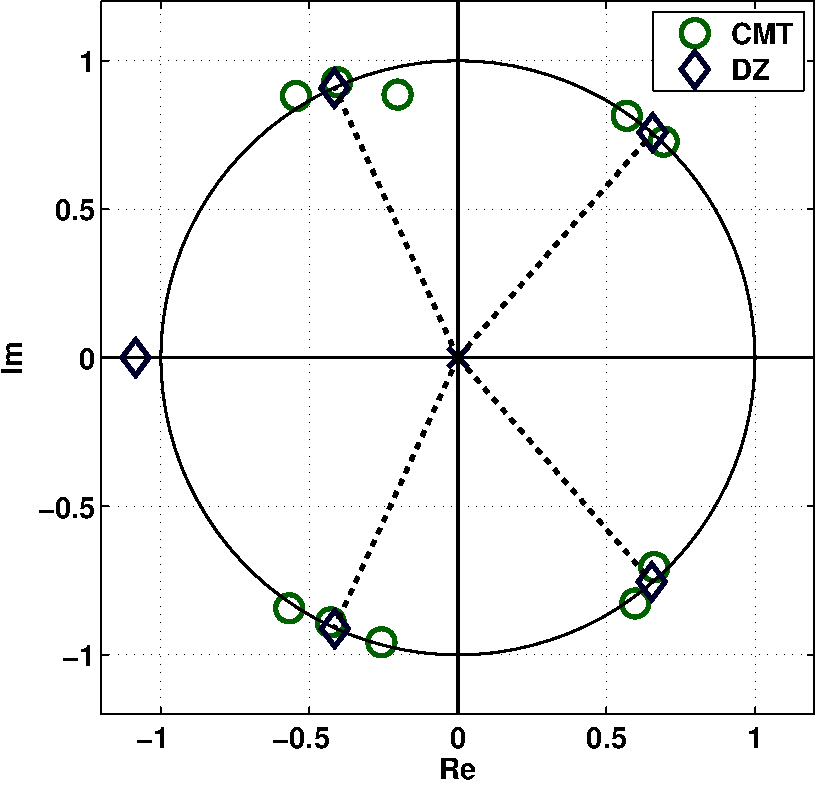
\includegraphics[width=3in]{./cmt_multi/cmt_pzplot_multi_D4.pdf}}
%   \caption{Zeros of CMT MVDR polynomial (green circles) and DZ MVDR
%     polynomial (black diamonds). The CMT MVDR ABF uses multiple zeros
%     at each interferer direction, depending on the chosen notch
%     width. The DZ MVDR ABF always uses two zero per interferer.}
% \label{fig:cmt-zeros-multi}
% \end{figure*}

% The
% DZ MVDR ABF consistently achieves lower output power under same
% conditions as observed in \figurename{}~\ref{fig:cmt-output-multi}.



% % Make clear that L snapshots are used to compute the weights first. Then we look at the output power over the same interval using the ECM for each instance.

% \subsection{Computational gain}
% \label{sec:computational-gain}
% \figurename{}\ref{fig:comp-gain} compares the computation time
% required by DZ MVDR (diamond markers) and SMI MVDR ABF (circle
% markers) implemented using ULAs with number of sensors ranging from
% $N = 11$ to $101$. The computation time for each ULA size was averaged
% over 3000 Monte Carlo experiments. Each experiment assumed $L = 2N$
% snapshots were available to implement the ABFs. DZ MVDR ABF clearly
% requires less computation time compared to the SMI MVDR ABF. The gain
% is more significant for longer arrays.

% % TODO: Consider including comp time for UC DZ MVDR to show that it
% % takes up more time than SMI MVDR.

% \begin{figure}[!t]
%   \centering
%   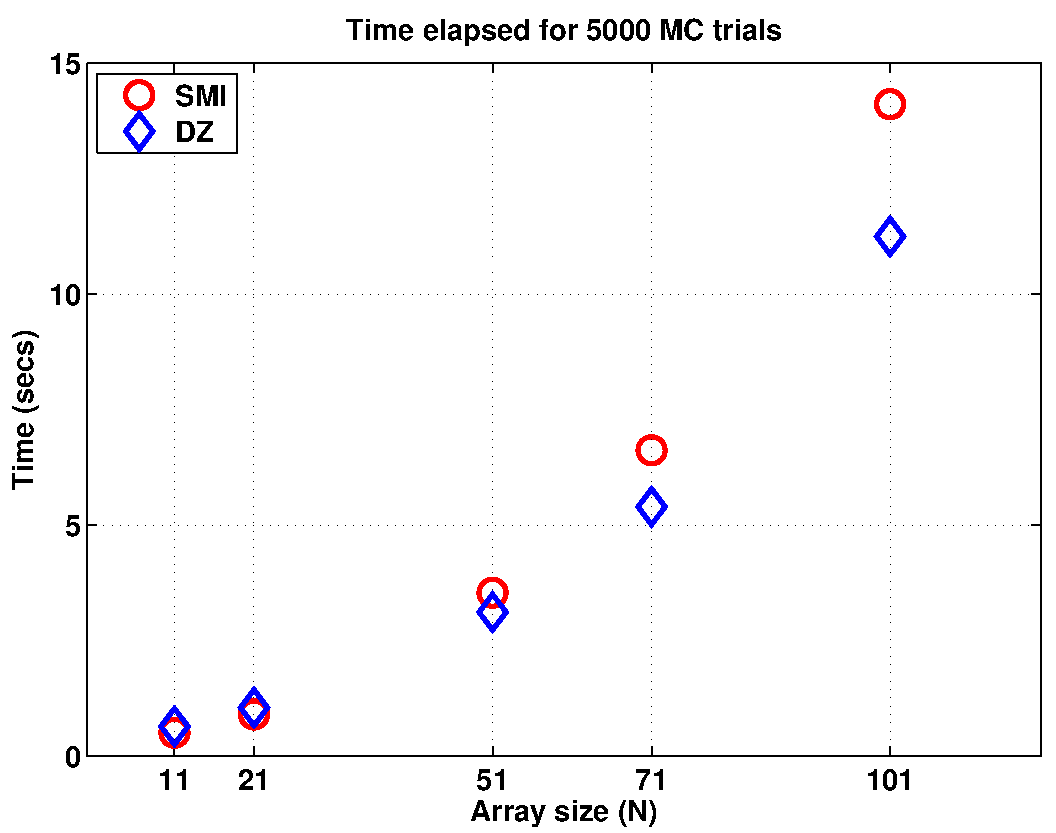
\includegraphics[width=2.5in]{comp_gain.pdf}
%   \caption{Computational gain using DZ MVDR over SMI MVDR.}
%   \label{fig:comp-gain}
% \end{figure}

%%% Local Variables:
%%% mode: latex
%%% TeX-master: "main"
%%% End:
  % result discussion
% ==========================================

\section{Summary}
\label{sec:dzmvdr-summary}
In conclusion, this chapter presents the DZ MVDR ABF which produces
a broad notch in the beampattern in the interferer direction. The DZ
MVDR ABF doubles the array polynomial zeros of a subarray SMI MVDR ABF
to derive the weight vector. The DZ MVDR ABF with the inherent
subarray processing requires less computation compared to the SMI MVDR
ABF implemented using same sized ULA. But the gain from subarray
processing is at the cost of reduced DOF and a wider main-lobe than the
SMI MVDR or the DL MVDR ABFs. Numerical experiments show that the DZ
MVDR ABF suppresses interferers better than both the SMI MVDR and the
DL MVDR ABF in the multiple stationary interferer scenario. Comparison
of the WNG shows that on average the DZ MVDR ABF has higher WNG making
it less sensitive to parameter mismatch. In moving interferer
scenarios, the DZ MVDR ABF performance is comparable to the CMT MVDR
ABF with the width parameter set equal to the ULA resolution
width. But the CMT MVDR requires choosing the width parameter while
the DZ MVDR ABF does not require making prior choice of design
parameters.

%%% Local Variables: 
%%% mode: latex
%%% TeX-master: "main"
%%% End: 
